\input{preamble}

\begin{document}

\begin{flushright}
Laura Fields\\
Paul Lebrun \\
Seongtae Park \\
Add more here \\
\today
\end{flushright}

%title
\begin{center}

{\LARGE LBNE Beam Alignment Tolerances}
\end{center}

%\tableofcontents

%\begin{abstract} 	

%\end{abstract}
\section{Introduction}

This note describes a study of LBNE beamline alignment tolerances and systematic uncertainties that was conducted in the winter of 2013-2014.  For each major source of beam alignment uncertainty (listed in Table~\ref{tab:syslist}), we evaluate the systematic uncertainty on the unoscillated muon neutrino flux assuming the nominal tolerances listed in Table~\ref{tab:syslist}.   The note is organized as follows: Section~\ref{sec:beamsim} describes the simulation used to execute the study; the procedure for extracting systematic uncertainties is summarized in Section~\ref{sec:procedure}, and the results are summarized in Section~\ref{sec:results}.  Plots showing the neutrino flux in various beam configuraitons and the fits used to extract systematic uncertainties are available in Appendix~\ref{app:plots}

\begin{table}
\centering
\begin{tabular}{ | c | c | }
\hline
  Target position (each end) & 0.5 mm \\
  Horn 1 position (each end) & 0.5 mm \\
  Horn 2 position (each end) & 0.5 mm \\
  Far detector position & 21 m \\
  Decay pipe position & 20 mm \\
  Decay pipe diameter & 0.1 m \\
  Horn current & 2 kA \\
  Horn water layer thickness & 0.5 mm \\
  Beam size at target & 0.1 mm \\
  Misalignment of shielding blocks & 1 cm \\
  Baffle scraping & 0.25\% \\
  Beam position at target & 0.45 mm \\
  Beam angle at target & 70 $\mu$rad \\
  Near detector position & 255 mm \\
  Horn conductor skin depth & 6 mm \\
  Target density & 2\% \\ 
\hline
\end{tabular}
\caption{Sources of beam misalignment and their expected tolerances, which were obtained from the LBNE CDR~\cite{lbnecdr} where applicable and from conversations with beam experts otherwise.}
\label{tab:syslist}
\end{table}

\section{Description of Beam Simulation}
\label{sec:beamsim}

\section{Procedure for Evaluating Systematic Uncertainties}
\label{sec:procedure}

In all cases, we evaluate the uncertainty on the muon neutrino flux at the near detector, at the far detector, and on the near/far flux ratio between 0 and 10 GeV in bins of 0.5 GeV.  For most sources of alignment uncertainty, we follow the follwing procedure:

\begin{itemize}
\item The flux at the near and far detectors in the nominal beam configurations is estimated using the simulation described in Section~\ref{sec:beamsim}.
\item The near and far detector fluxes are also estimated for several values of a particular alignment quantity (e.g. offsets of Horn 1).  
\item The near detector flux, far detector flux and near/far flux ratio are plotted as a function of the misaligned quantity.  
\item In each 0.5 GeV energy bin,  the dependence of the near, far and near/far fluxes on the amount of misalignment is extracted using fits that assume either a linear or a parabolic dependence of the flux in each energy bin on the amount of misalignment. 
\item The systematic uncertainty is extracted from the fit functions evaluated at the tolerance of quantity in question (listed in Table~\ref{tab:syslist}).  The linear or parabolic fit is chosen based on which has the lowest $\chi^2$ value.
\end{itemize}

This procedure, which closely follows a similar study performed for the NuMI beamline~\cite{numitdh}, is used to evaluate all of the alignment uncertainties listed in Table~\ref{tab:syslist} except for baffle scraping and shielding block alignment. An example is shown in Figure~\ref{fig:TargetXOffset_nof_summary}, where the the points show the fractional change in the near over far flux ratio for various shifts of the target position along the x axis.  The fits to each energy bin are shown in Figure~\ref{fig:TargetXOffset_nof_fits}, and the results of the fit are shown by the solid lines in Figure~\ref{fig:TargetXOffset_nof_summary}.  The total error, estimated by evaluating the fits at the target position tolerance of 0.5 mm, is shown in Figure~\ref{fig:TargetXOffset_nof_error}.

\begin{figure}[ht]
\label{fig:TargetXOffset_nof_summary}
  \begin{center}
    {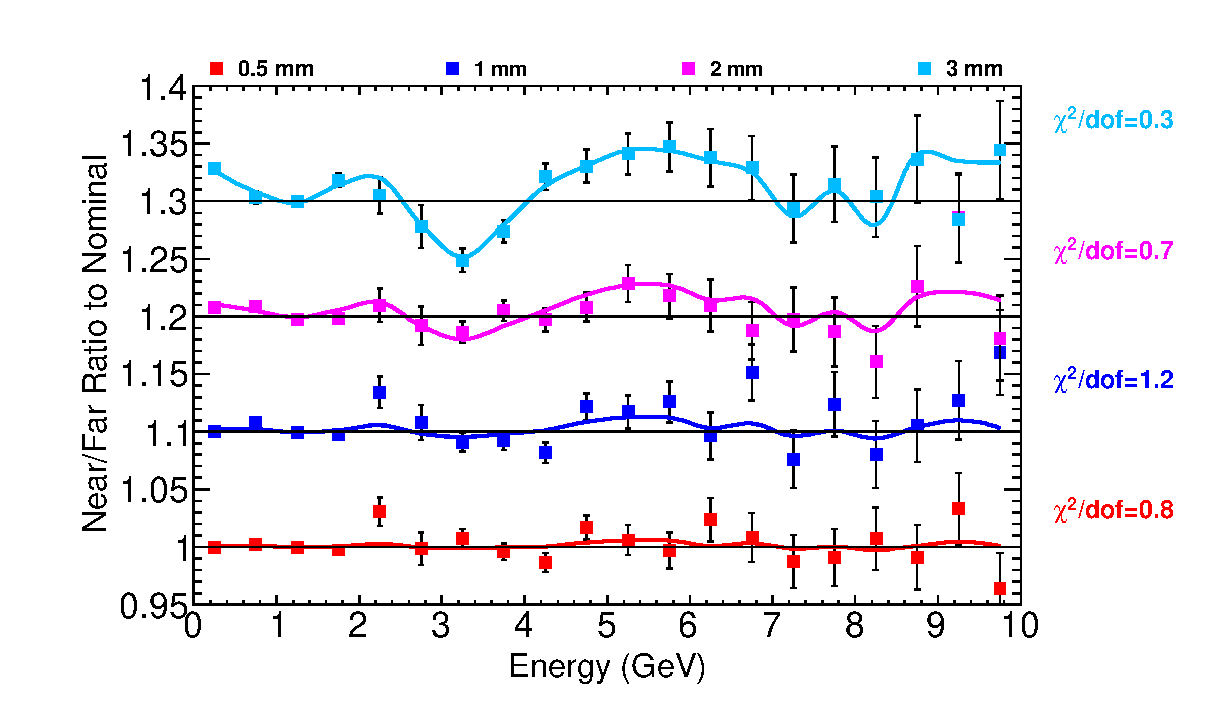
\includegraphics[width=6.0in]{figures/TargetXOffset_nof_summary.eps}}
  \end{center}
\caption{ Near/Far double ratios to nominal for several values of {\bf Target Offset in $x$} (points) and the results of the fits to each energy bin (lines).}
\end{figure}

\begin{figure}[ht]
\label{fig:TargetXOffset_nof_fits}
  \begin{center}
    {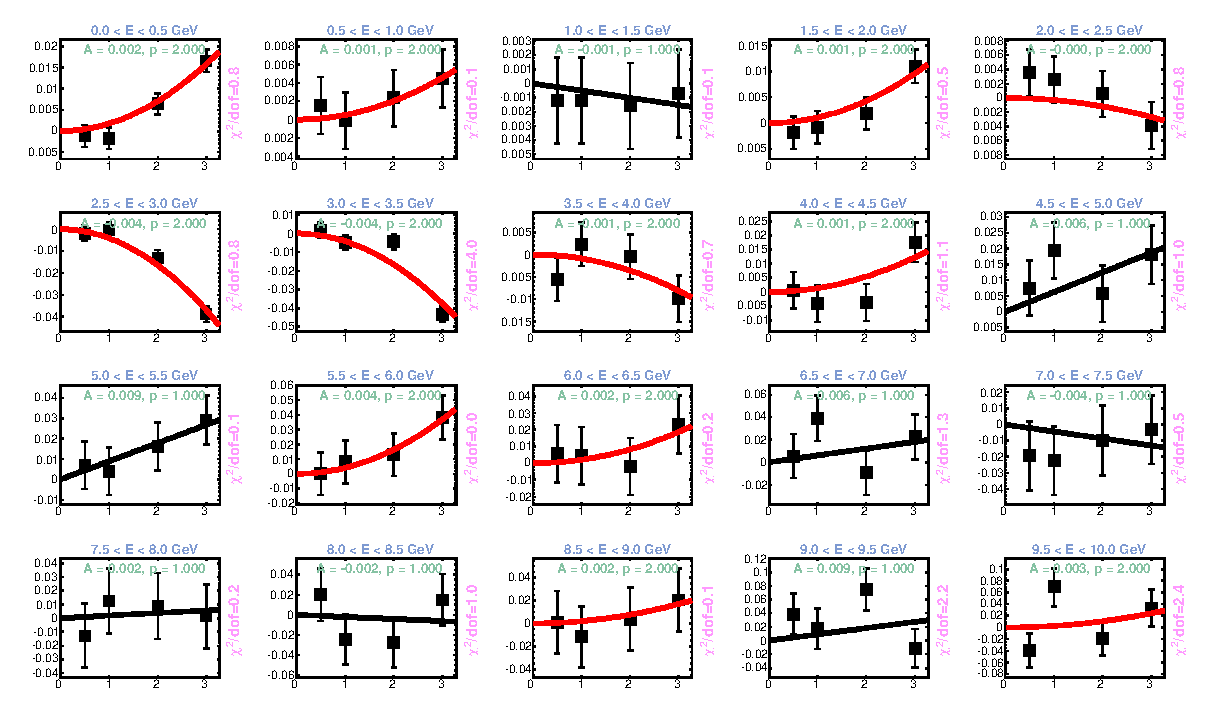
\includegraphics[width=5.0in]{figures/TargetXOffset_nof_fits.eps}}
  \end{center}
\caption{ Fits to the near/far ratios for several values of {\bf Target Offset in $x$}. Black(Red) fit lines indicate that a linear(parabolic) fit provided the best $\chi^2$. }
\end{figure}

\begin{figure}[ht]
\label{fig:TargetXOffset_nof_error}
  \begin{center}
    {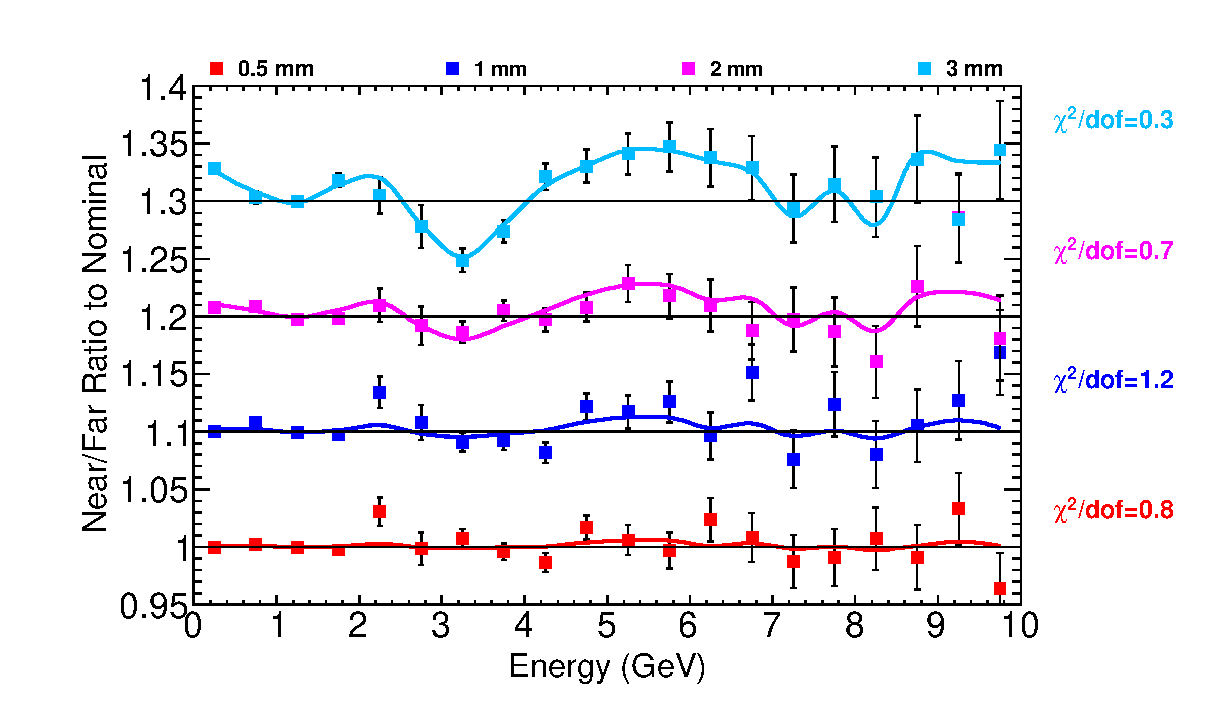
\includegraphics[width=6.0in]{figures/TargetXOffset_nof_summary.eps}}
  \end{center}
\caption{ Near/Far double ratios to nominal for several values of {\bf Target Offset in $x$} (points) and the results of the fits to each energy bin (lines).}
\end{figure}


To study the effect of shielding block alignment, we have simlated the flux with and without shielding blocks present and find no difference from the nominal configuration beyond statistical fluctuations.  We therefore assume that alignment block shifts of order 1 cm would lead to negligible systematic uncertainties and do not include this source in our total estimat of alignment uncertainties.

For the baffle scraping uncertainty, we estimate the flux from the baffle by simulating a point-like beam fired directly at the baffle. Specifically, we simulate a beam with a 0.001 mm standard deviation in width and height offset from the origin by 7 mm.  We then estimate baffle uncertainty by adding 0.25% (the baffle scraping tolerance) of the baffle flux to the nominal flux.  

\section{Results}
\label{sec:results}

\section{Conclusion}

\appendix
\section{Flux Variation and Fit Plots}
\label{app:plots}

\vspace{3in}


\begin{figure}[ht]
  \begin{center}
    {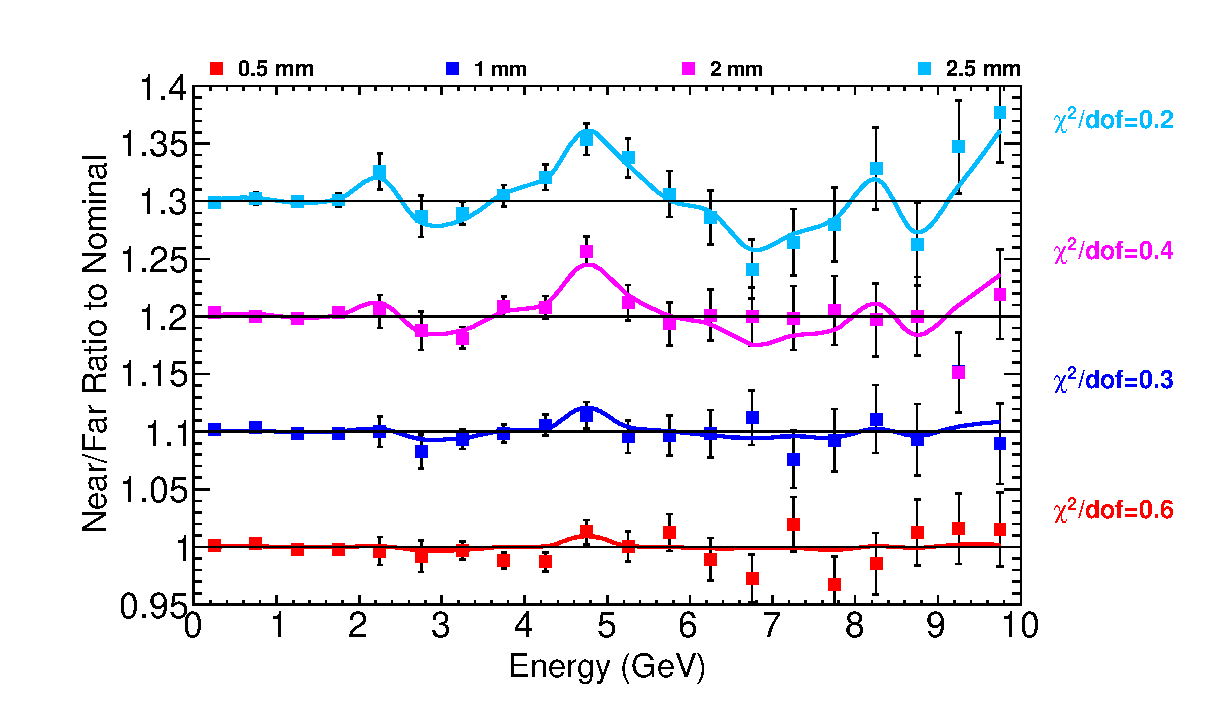
\includegraphics[width=6.0in]{figures/Horn1XOffset_nof_summary.eps}}
  \end{center}
\caption{ Near/Far double ratios to nominal for several values of {\bf Horn 1 Offset in $x$} (points) and the results of the fits to each energy bin (lines).}
\end{figure}

\begin{figure}[ht]
  \begin{center}
    {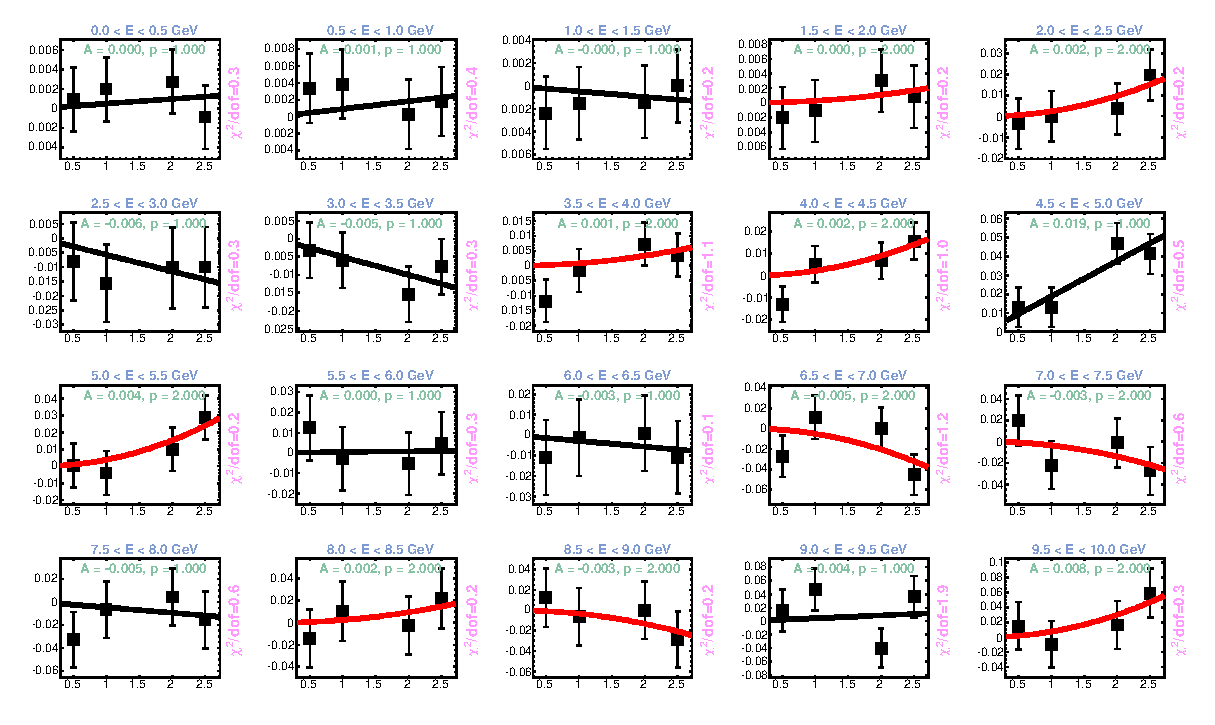
\includegraphics[width=5.0in]{figures/Horn1XOffset_nof_fits.eps}}
  \end{center}
\caption{ Fits to the near/far ratios for several values of {\bf Horn 1 Offset in $x$}. Black(Red) fit lines indicate that a linear(parabolic) fit provided the best $\chi^2$. }
\end{figure}

\begin{figure}[ht]
  \begin{center}
    {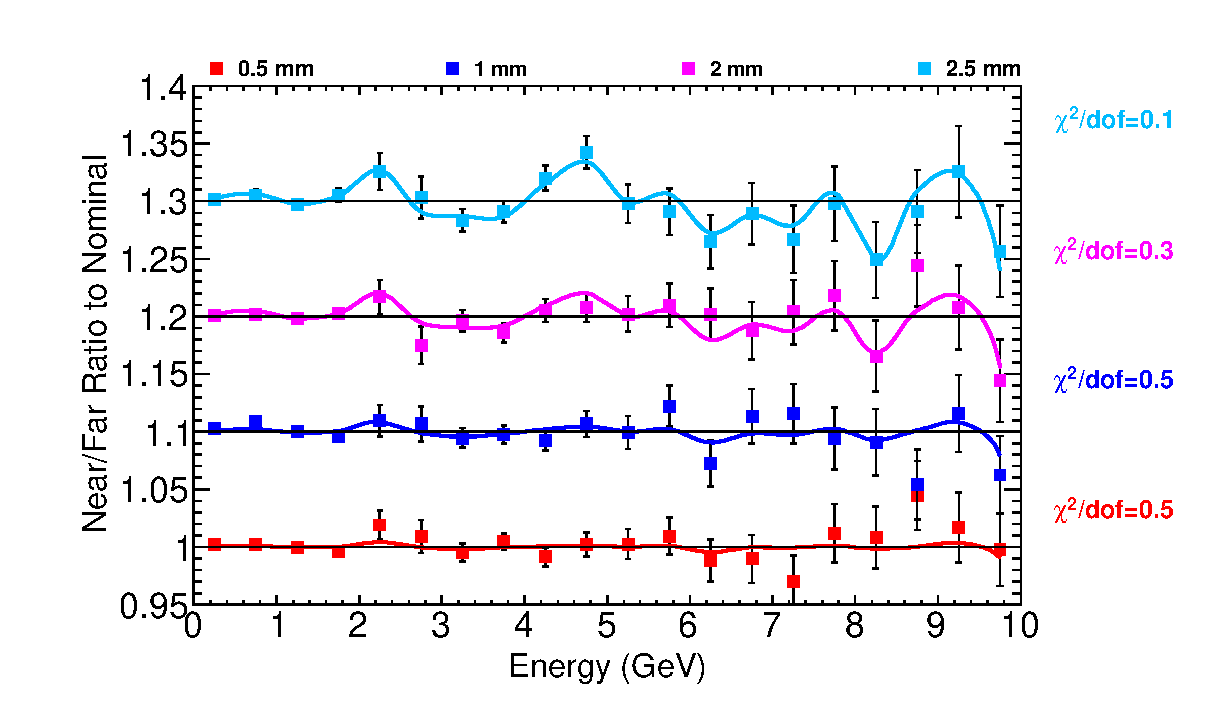
\includegraphics[width=6.0in]{figures/Horn1YOffset_nof_summary.eps}}
  \end{center}
\caption{ Near/Far double ratios to nominal for several values of {\bf Horn 1 Offset in $y$} (points) and the results of the fits to each energy bin (lines).}
\end{figure}

\begin{figure}[ht]
  \begin{center}
    {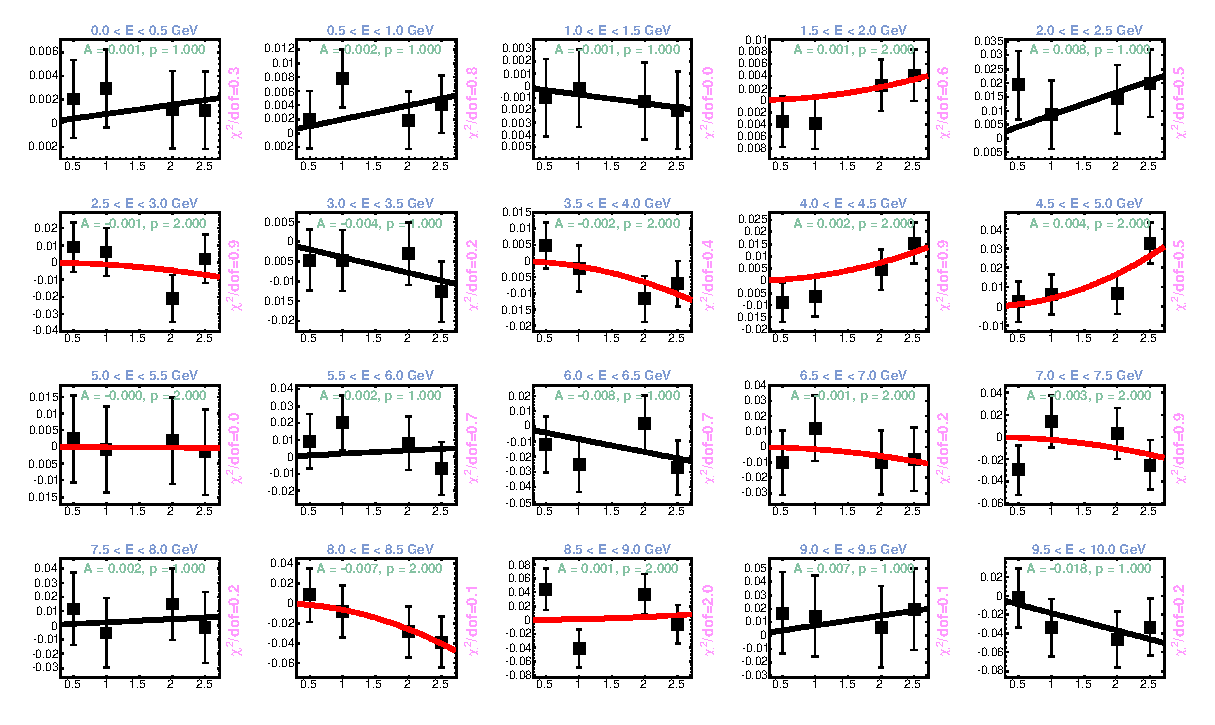
\includegraphics[width=5.0in]{figures/Horn1YOffset_nof_fits.eps}}
  \end{center}
\caption{ Fits to the near/far ratios for several values of {\bf Horn 1 Offset in $y$}. Black(Red) fit lines indicate that a linear(parabolic) fit provided the best $\chi^2$. }
\end{figure}

\begin{figure}[ht]
  \begin{center}
    {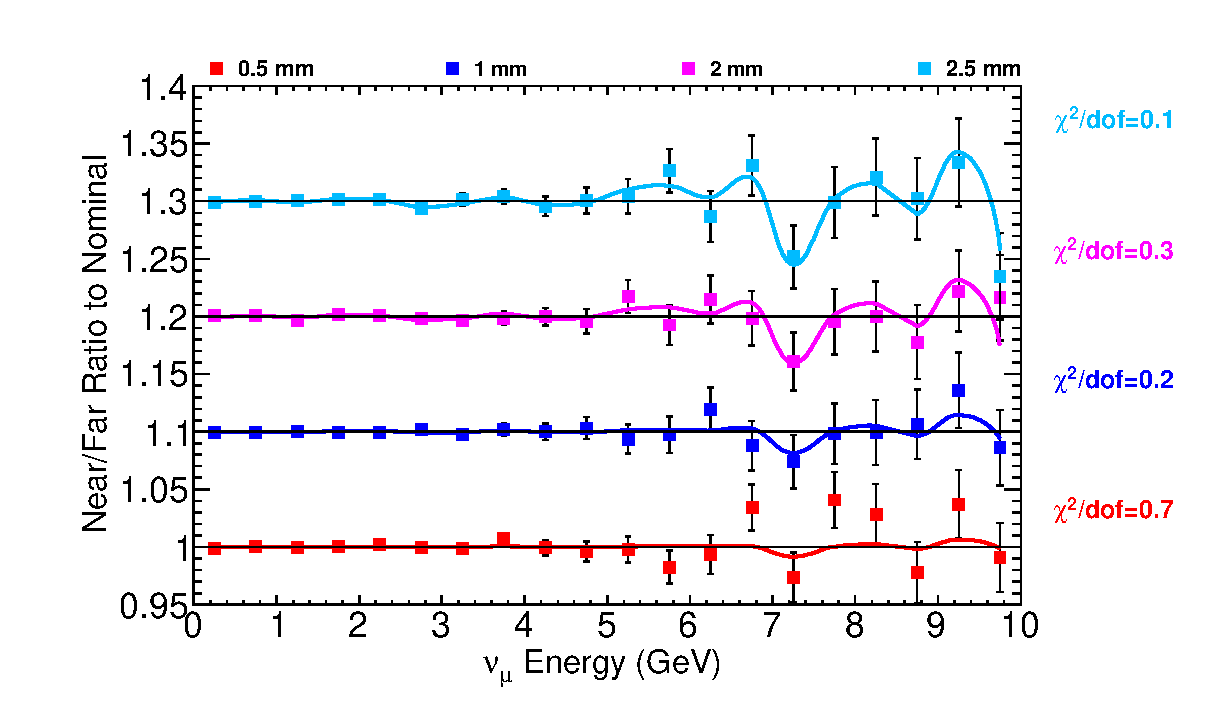
\includegraphics[width=6.0in]{figures/Horn2XOffset_nof_summary.eps}}
  \end{center}
\caption{ Near/Far double ratios to nominal for several values of {\bf Horn 2 Offset in $x$} (points) and the results of the fits to each energy bin (lines).}
\end{figure}

\begin{figure}[ht]
  \begin{center}
    {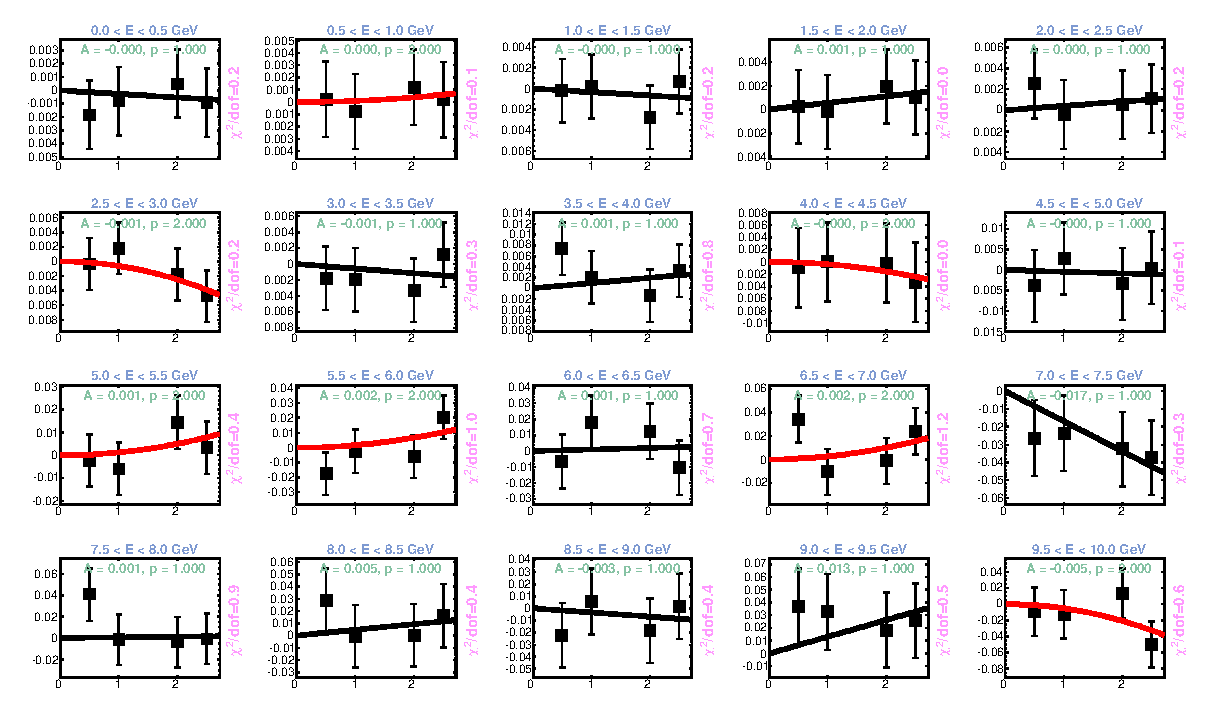
\includegraphics[width=5.0in]{figures/Horn2XOffset_nof_fits.eps}}
  \end{center}
\caption{ Fits to the near/far ratios for several values of {\bf Horn 2 Offset in $x$}. Black(Red) fit lines indicate that a linear(parabolic) fit provided the best $\chi^2$. }
\end{figure}

\begin{figure}[ht]
  \begin{center}
    {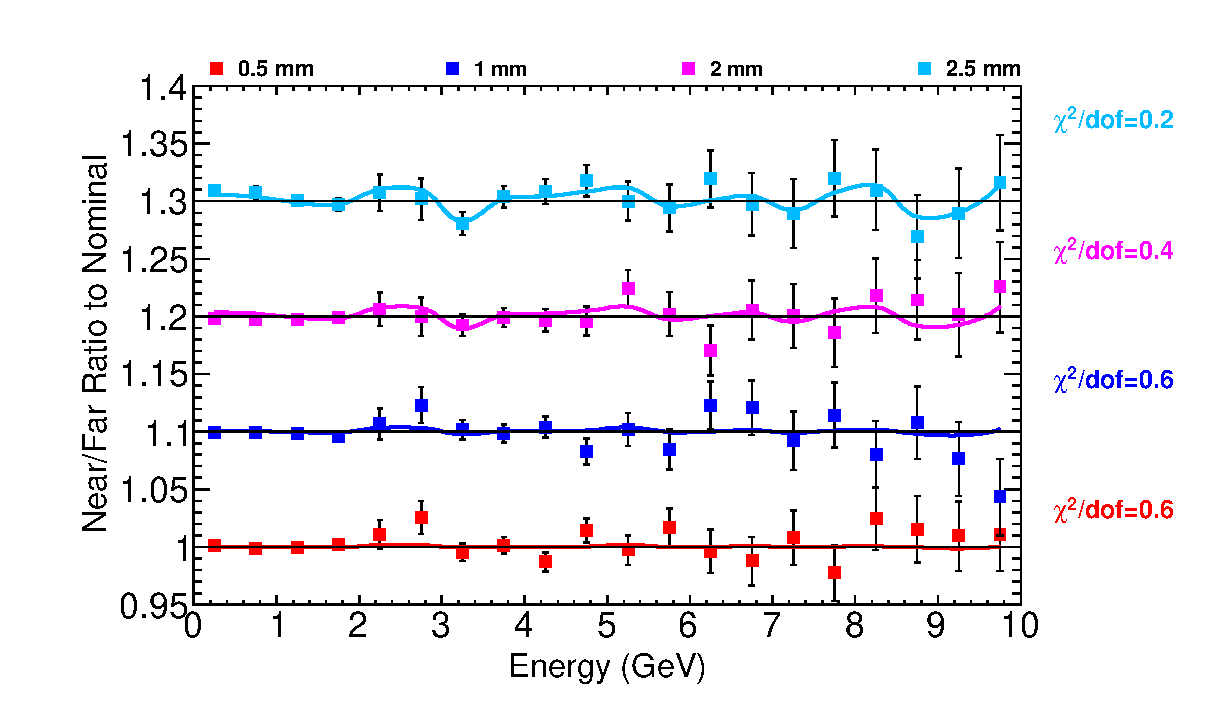
\includegraphics[width=6.0in]{figures/Horn2YOffset_nof_summary.eps}}
  \end{center}
\caption{ Near/Far double ratios to nominal for several values of {\bf Horn 2 Offset in $y$} (points) and the results of the fits to each energy bin (lines).}
\end{figure}

\begin{figure}[ht]
  \begin{center}
    {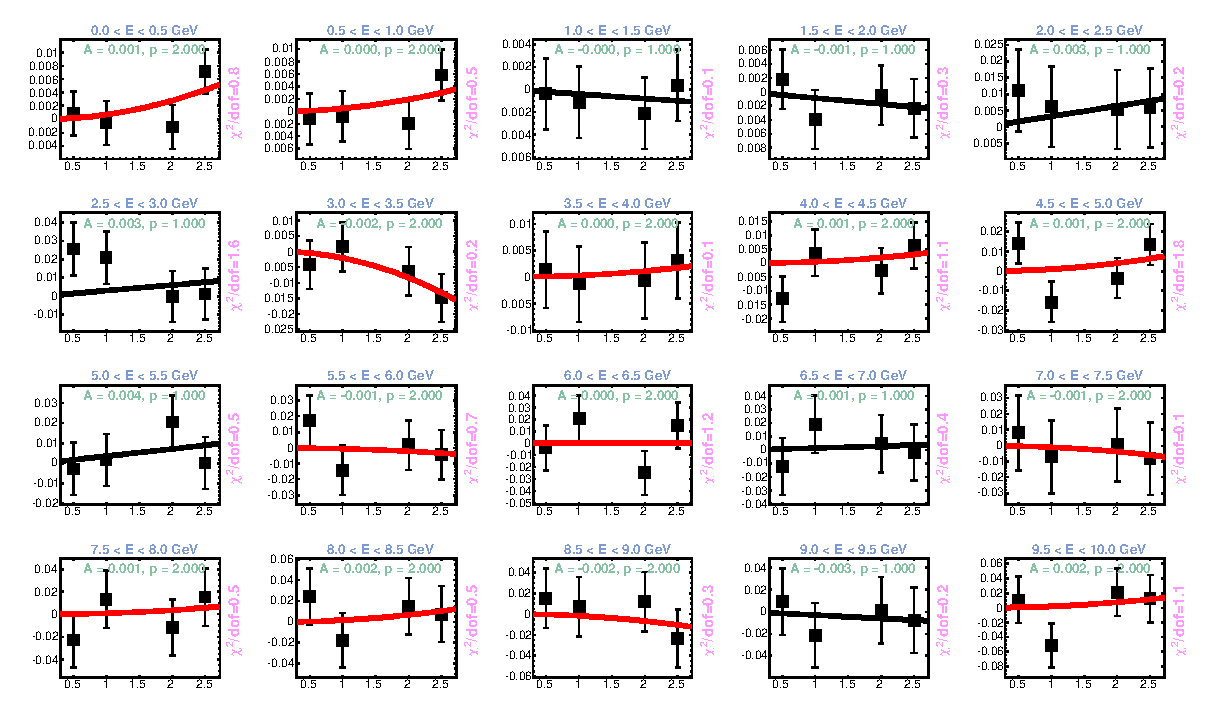
\includegraphics[width=5.0in]{figures/Horn2YOffset_nof_fits.eps}}
  \end{center}
\caption{ Fits to the near/far ratios for several values of {\bf Horn 2 Offset in $y$}. Black(Red) fit lines indicate that a linear(parabolic) fit provided the best $\chi^2$. }
\end{figure}

\begin{figure}[ht]
  \begin{center}
    {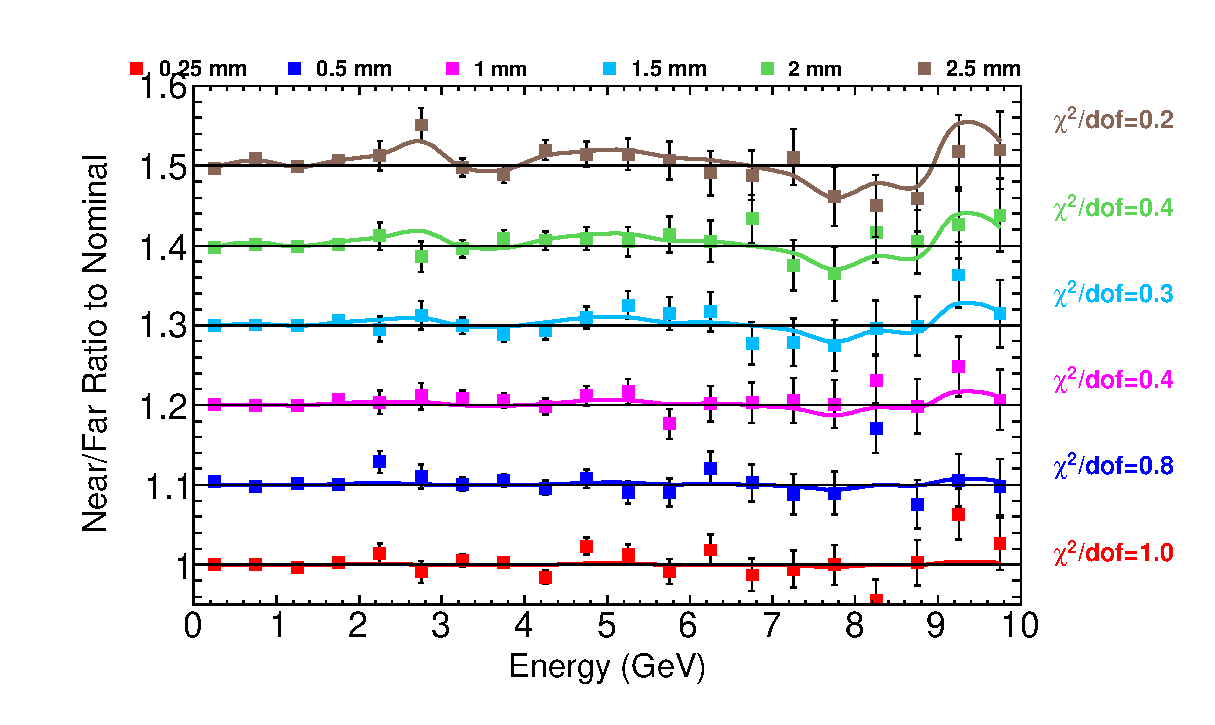
\includegraphics[width=6.0in]{figures/Horn1XTilt_nof_summary.eps}}
  \end{center}
\caption{ Near/Far double ratios to nominal for several values of {\bf Horn 1 Tilt in $x$} (points) and the results of the fits to each energy bin (lines).}
\end{figure}

\begin{figure}[ht]
  \begin{center}
    {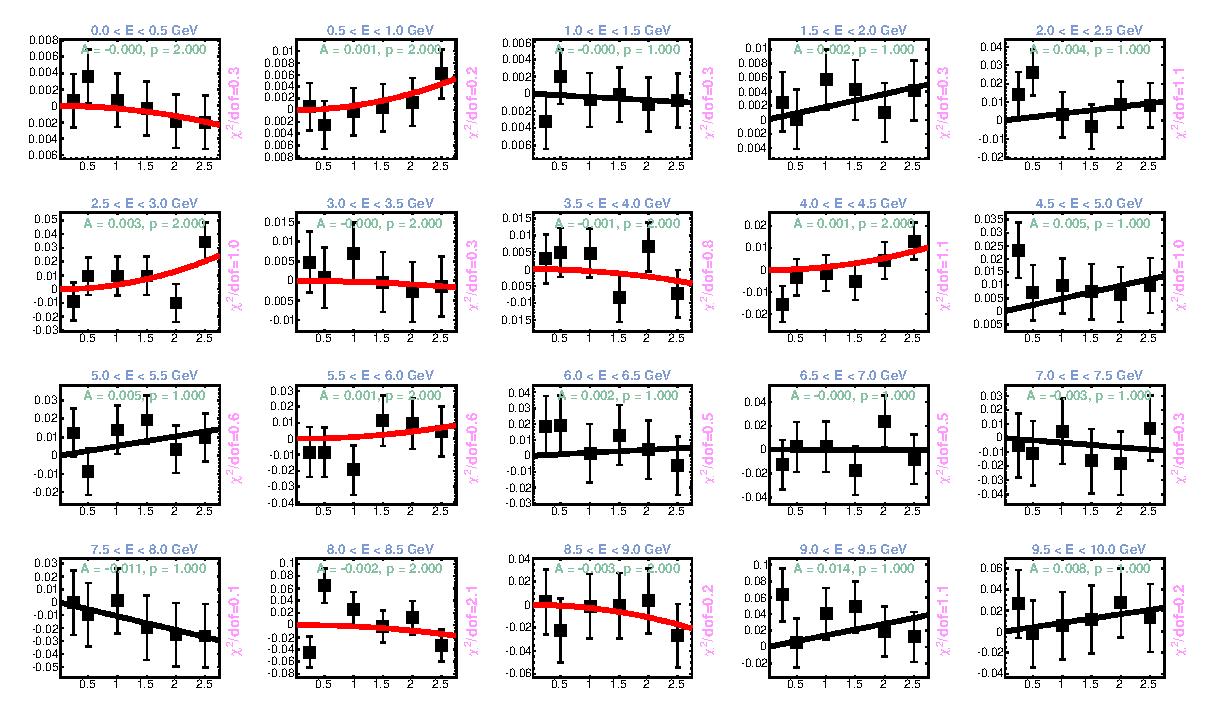
\includegraphics[width=5.0in]{figures/Horn1XTilt_nof_fits.eps}}
  \end{center}
\caption{ Fits to the near/far ratios for several values of {\bf Horn 1 Tilt in $x$}. Black(Red) fit lines indicate that a linear(parabolic) fit provided the best $\chi^2$. }
\end{figure}

\begin{figure}[ht]
  \begin{center}
    {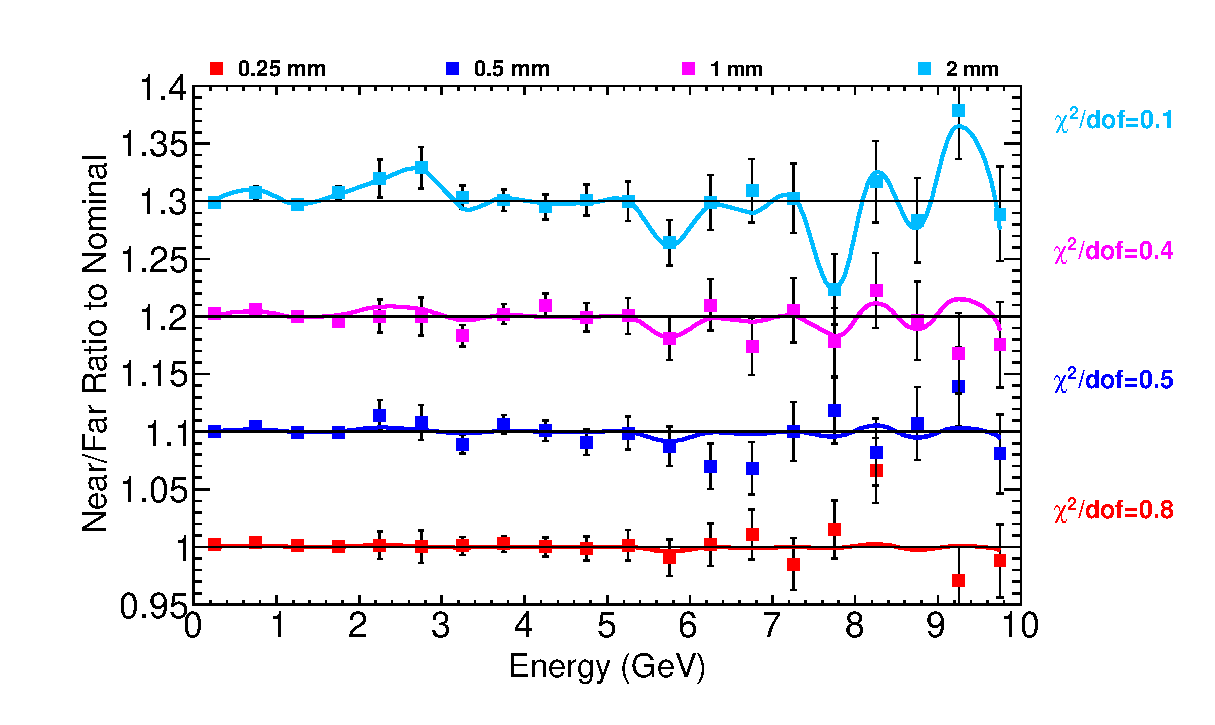
\includegraphics[width=6.0in]{figures/Horn1YTilt_nof_summary.eps}}
  \end{center}
\caption{ Near/Far double ratios to nominal for several values of {\bf Horn 1 Tilt in $y$} (points) and the results of the fits to each energy bin (lines).}
\end{figure}

\clearpage

\begin{figure}[ht]
  \begin{center}
    {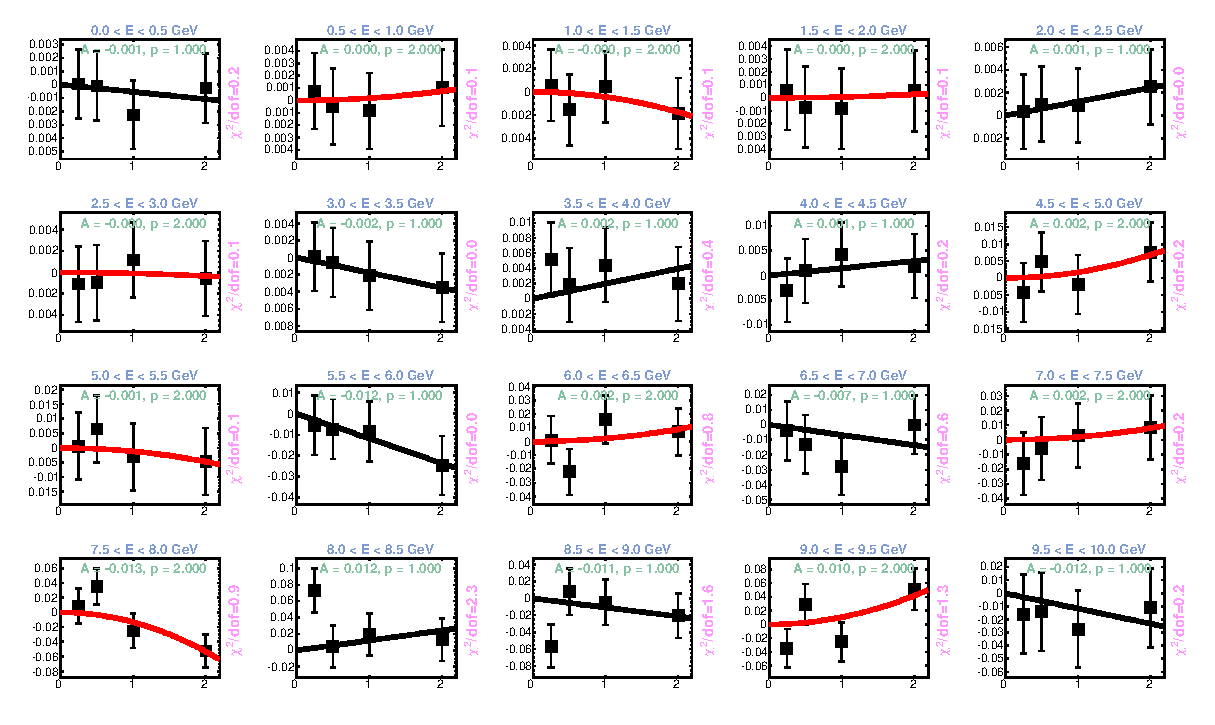
\includegraphics[width=5.0in]{figures/Horn1YTilt_nof_fits.eps}}
  \end{center}
\caption{ Fits to the near/far ratios for several values of {\bf Horn 1 Tilt in $y$}. Black(Red) fit lines indicate that a linear(parabolic) fit provided the best $\chi^2$. }
\end{figure}



\begin{figure}[ht]
  \begin{center}
    {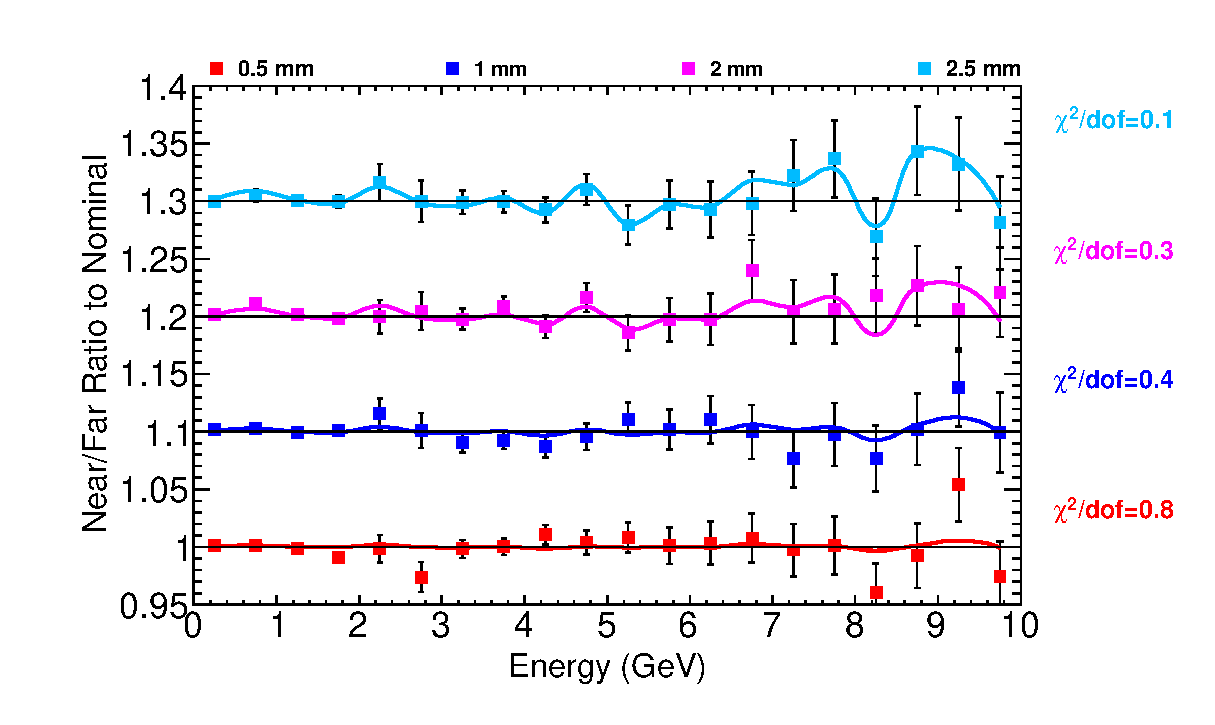
\includegraphics[width=6.0in]{figures/Horn2XTilt_nof_summary.eps}}
  \end{center}
\caption{ Near/Far double ratios to nominal for several values of {\bf Horn 2 Tilt in $x$} (points) and the results of the fits to each energy bin (lines).}
\end{figure}

\begin{figure}[ht]
  \begin{center}
    {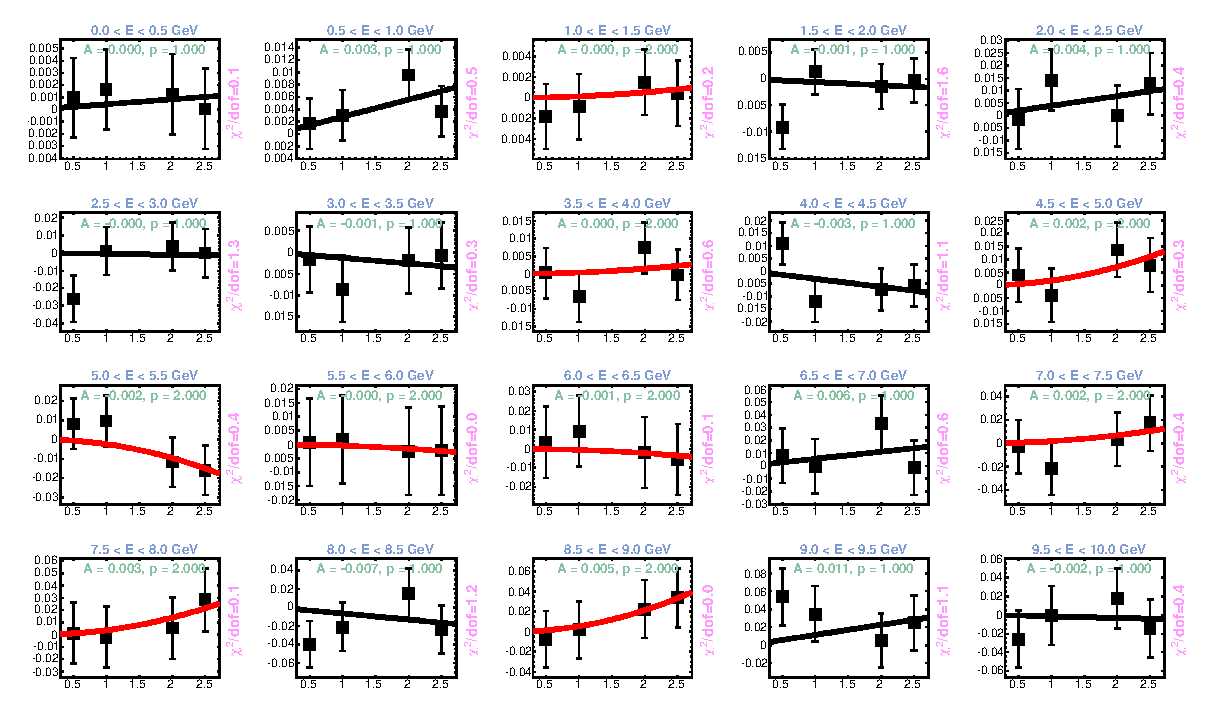
\includegraphics[width=5.0in]{figures/Horn2XTilt_nof_fits.eps}}
  \end{center}
\caption{ Fits to the near/far ratios for several values of {\bf Horn 2 Tilt in $x$}. Black(Red) fit lines indicate that a linear(parabolic) fit provided the best $\chi^2$. }
\end{figure}

\begin{figure}[ht]
  \begin{center}
    {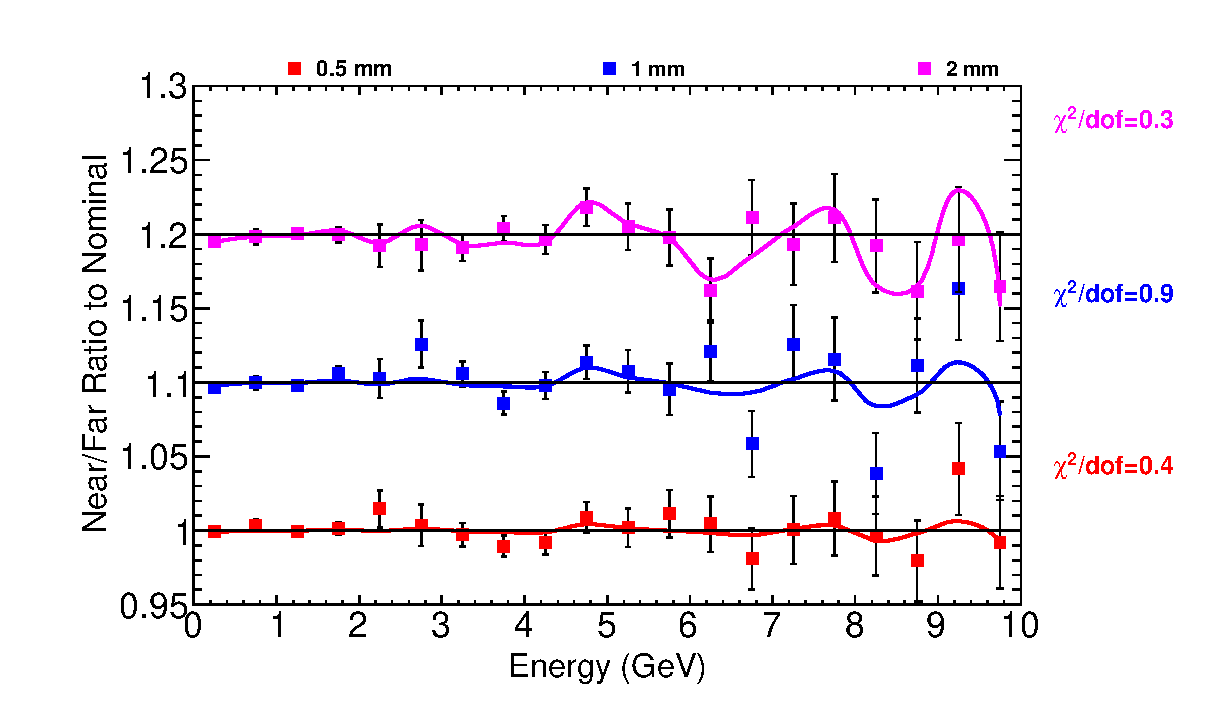
\includegraphics[width=6.0in]{figures/Horn2YTilt_nof_summary.eps}}
  \end{center}
\caption{ Near/Far double ratios to nominal for several values of {\bf Horn 2 Tilt in $y$} (points) and the results of the fits to each energy bin (lines).}
\end{figure}

\begin{figure}[ht]
  \begin{center}
    {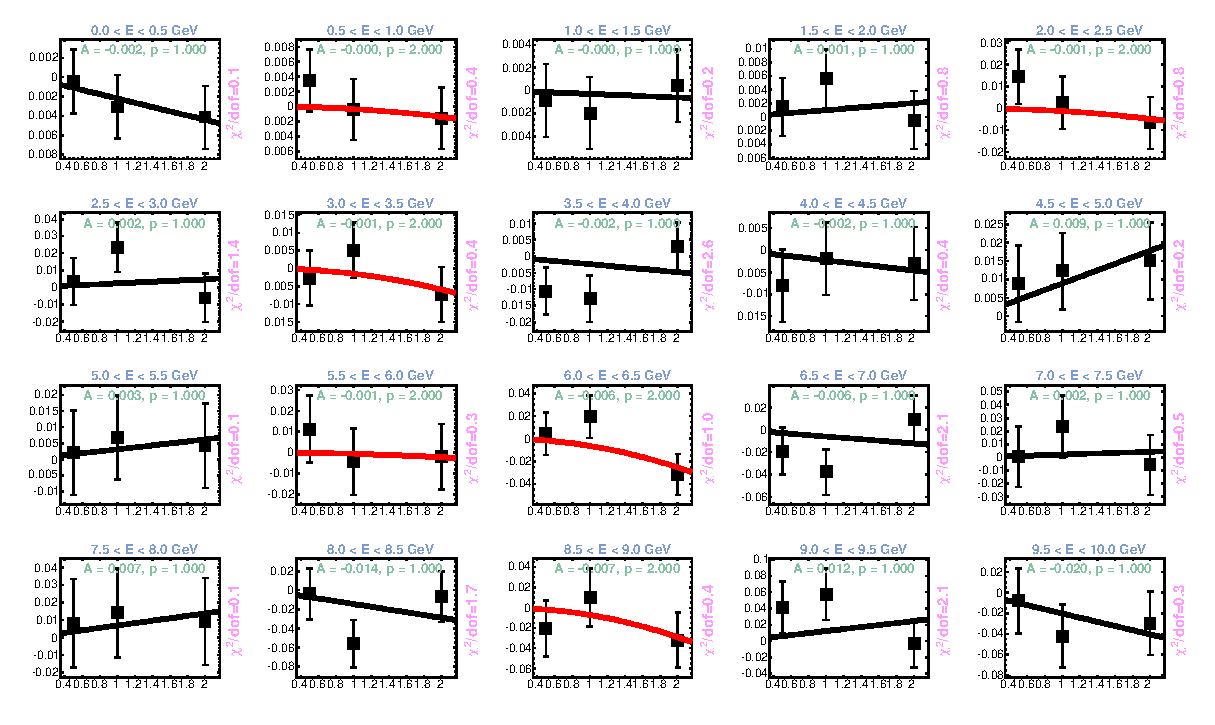
\includegraphics[width=5.0in]{figures/Horn2YTilt_nof_fits.eps}}
  \end{center}
\caption{ Fits to the near/far ratios for several values of {\bf Horn 2 Tilt in $y$}. Black(Red) fit lines indicate that a linear(parabolic) fit provided the best $\chi^2$. }
\end{figure}

\begin{figure}[ht]
  \begin{center}
    {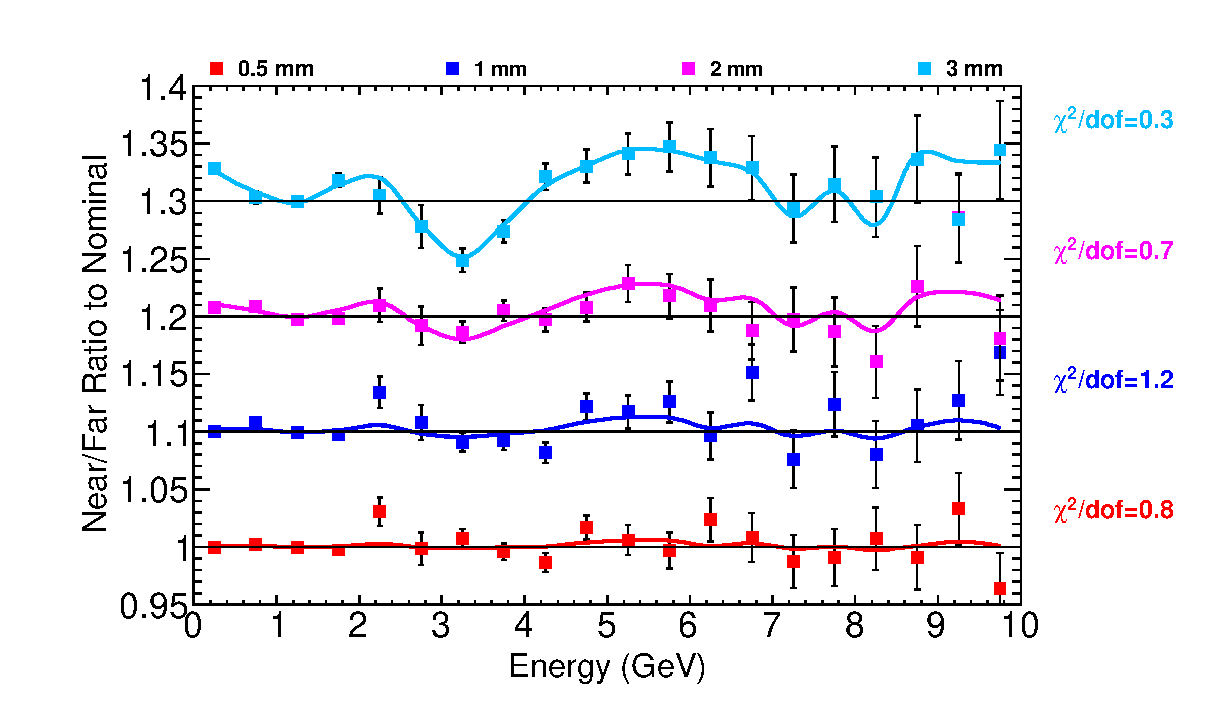
\includegraphics[width=6.0in]{figures/TargetXOffset_nof_summary.eps}}
  \end{center}
\caption{ Near/Far double ratios to nominal for several values of {\bf Target Offset in $x$} (points) and the results of the fits to each energy bin (lines).}
\end{figure}

\begin{figure}[ht]
  \begin{center}
    {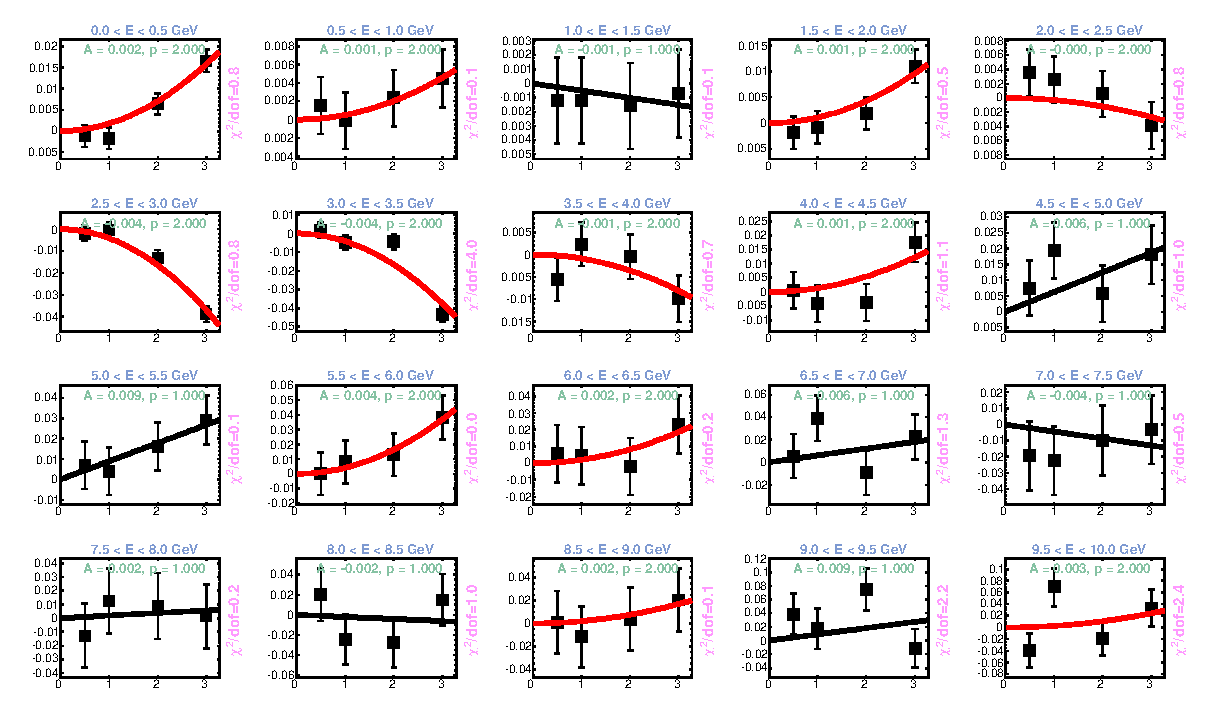
\includegraphics[width=5.0in]{figures/TargetXOffset_nof_fits.eps}}
  \end{center}
\caption{ Fits to the near/far ratios for several values of {\bf Target Offset in $x$}. Black(Red) fit lines indicate that a linear(parabolic) fit provided the best $\chi^2$. }
\end{figure}

\begin{figure}[ht]
  \begin{center}
    {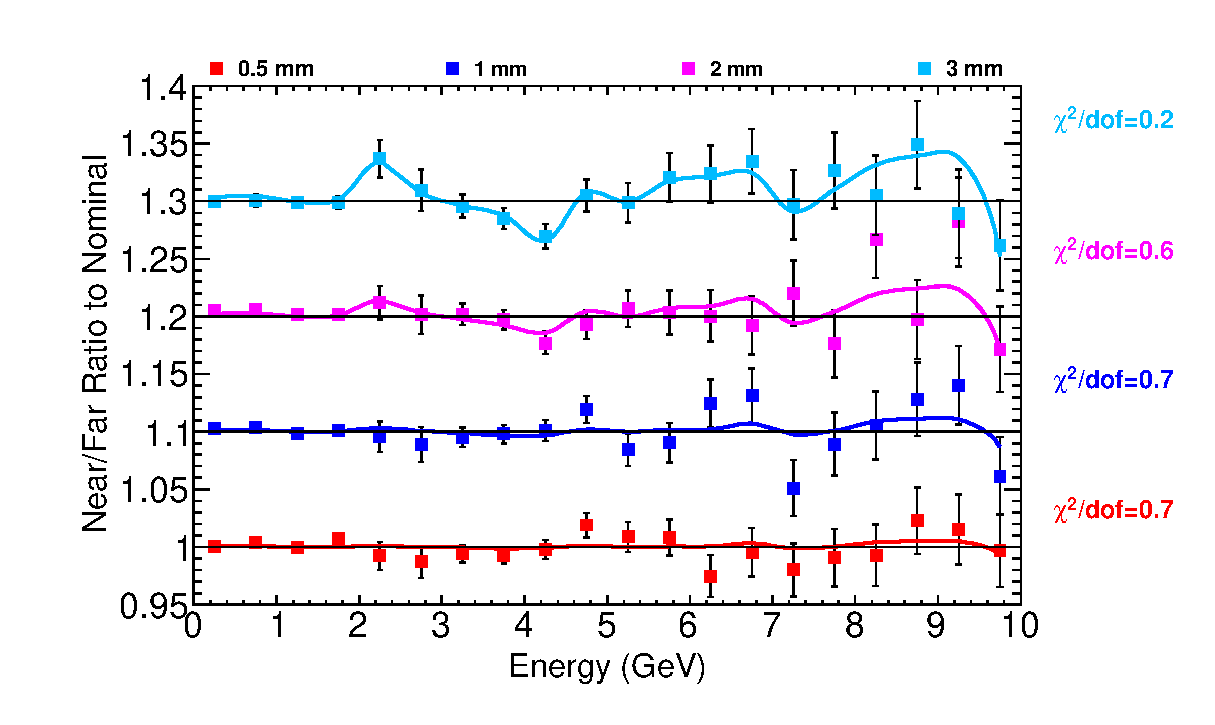
\includegraphics[width=6.0in]{figures/TargetYOffset_nof_summary.eps}}
  \end{center}
\caption{ Near/Far double ratios to nominal for several values of {\bf Target Offset in $y$} (points) and the results of the fits to each energy bin (lines).}
\end{figure}

\begin{figure}[ht]
  \begin{center}
    {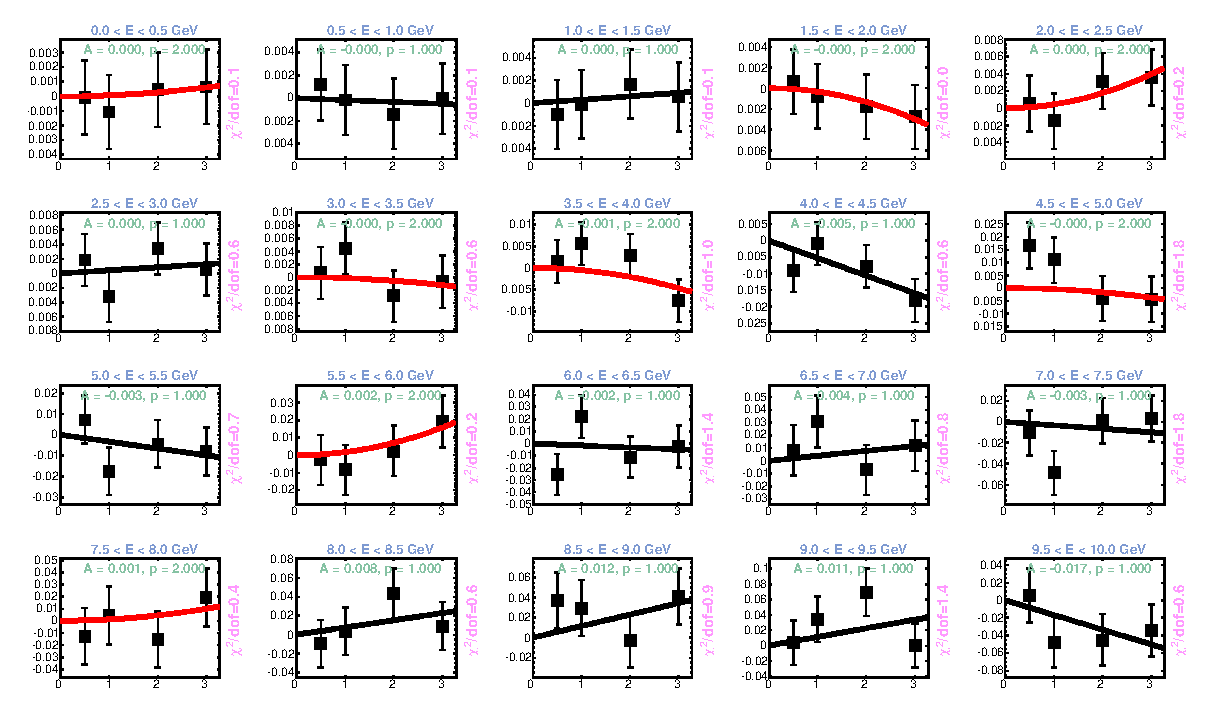
\includegraphics[width=5.0in]{figures/TargetYOffset_nof_fits.eps}}
  \end{center}
\caption{ Fits to the near/far ratios for several values of {\bf Target Offset in $y$}. Black(Red) fit lines indicate that a linear(parabolic) fit provided the best $\chi^2$. }
\end{figure}

\begin{figure}[ht]
  \begin{center}
    {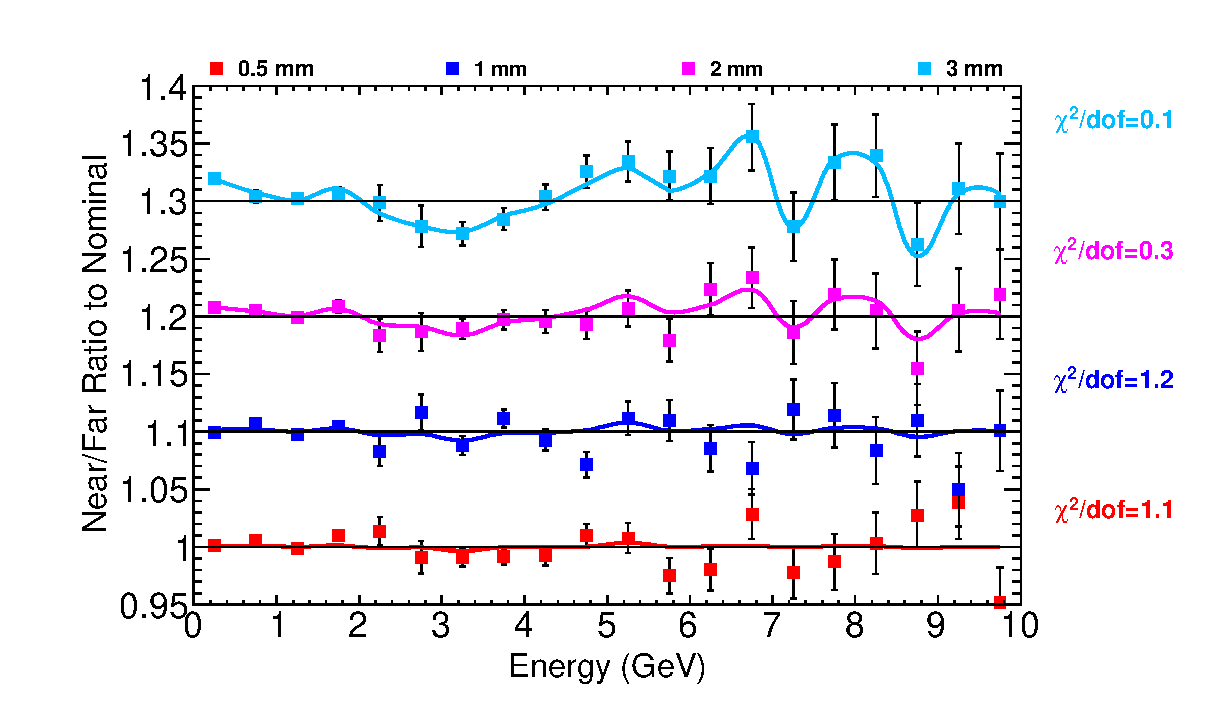
\includegraphics[width=6.0in]{figures/TargetXTilt_nof_summary.eps}}
  \end{center}
\caption{ Near/Far double ratios to nominal for several values of {\bf Target Tilt in $x$} (points) and the results of the fits to each energy bin (lines).}
\end{figure}

\begin{figure}[ht]
  \begin{center}
    {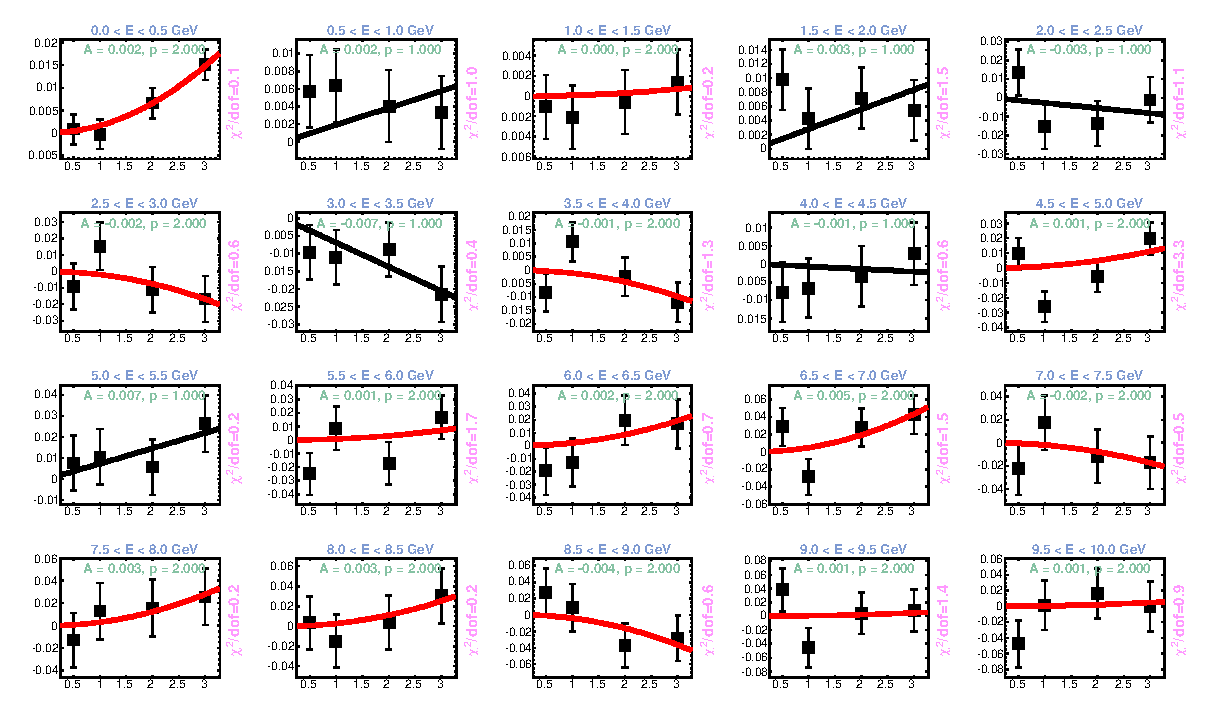
\includegraphics[width=5.0in]{figures/TargetXTilt_nof_fits.eps}}
  \end{center}
\caption{ Fits to the near/far ratios for several values of {\bf Target Tilt in $x$}. Black(Red) fit lines indicate that a linear(parabolic) fit provided the best $\chi^2$. }
\end{figure}

\clearpage

\begin{figure}[ht]
  \begin{center}
    {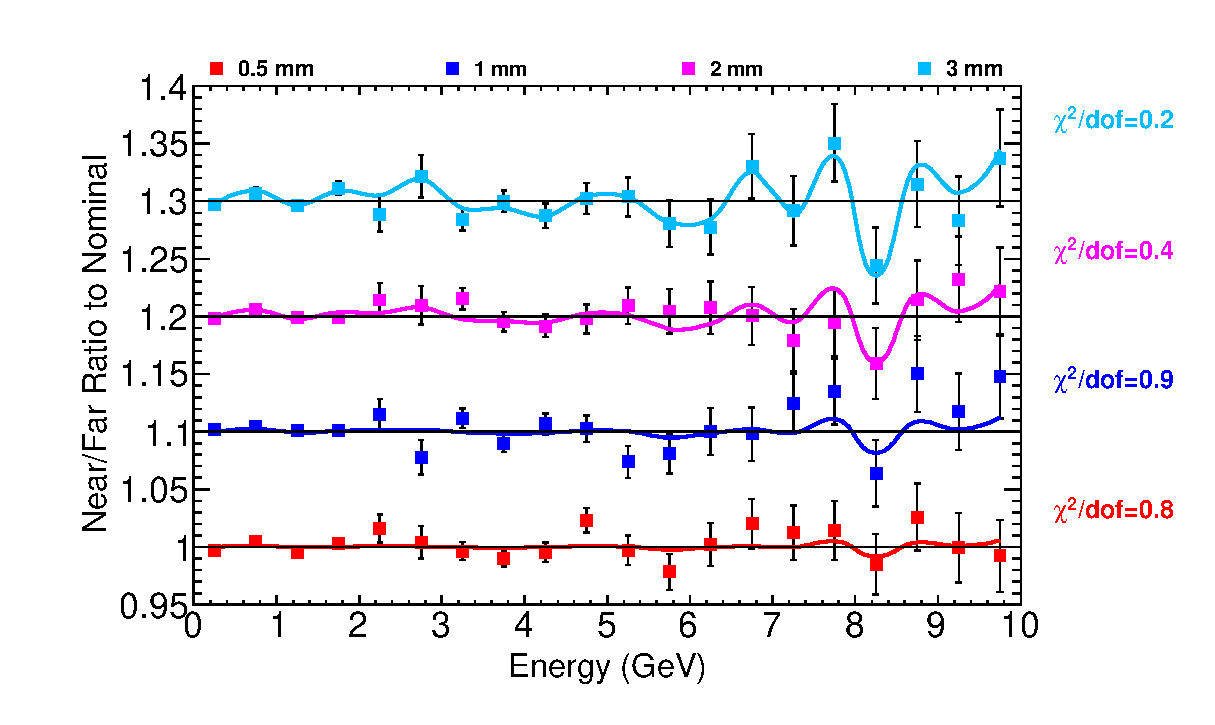
\includegraphics[width=6.0in]{figures/TargetYTilt_nof_summary.eps}}
  \end{center}
\caption{ Near/Far double ratios to nominal for several values of {\bf Target Tilt in $y$} (points) and the results of the fits to each energy bin (lines).}
\end{figure}

\begin{figure}[ht]
  \begin{center}
    {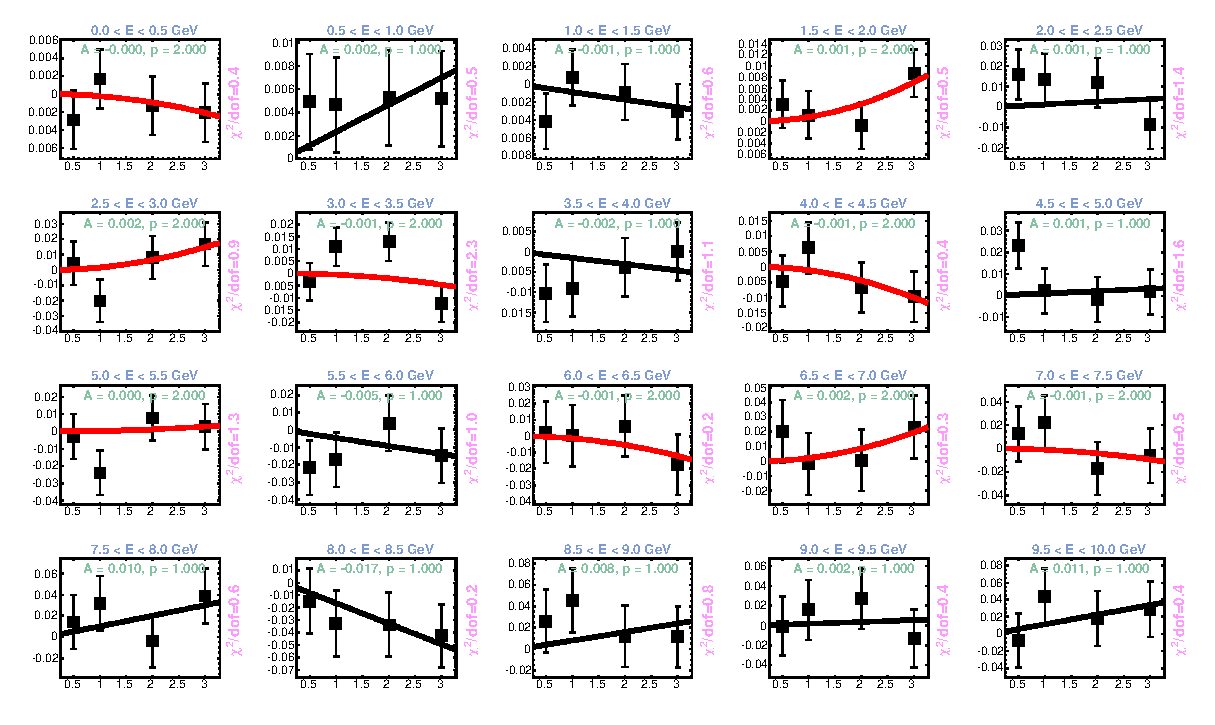
\includegraphics[width=5.0in]{figures/TargetYTilt_nof_fits.eps}}
  \end{center}
\caption{ Fits to the near/far ratios for several values of {\bf Target Tilt in $y$}. Black(Red) fit lines indicate that a linear(parabolic) fit provided the best $\chi^2$. }
\end{figure}


\begin{figure}[ht]
  \begin{center}
    {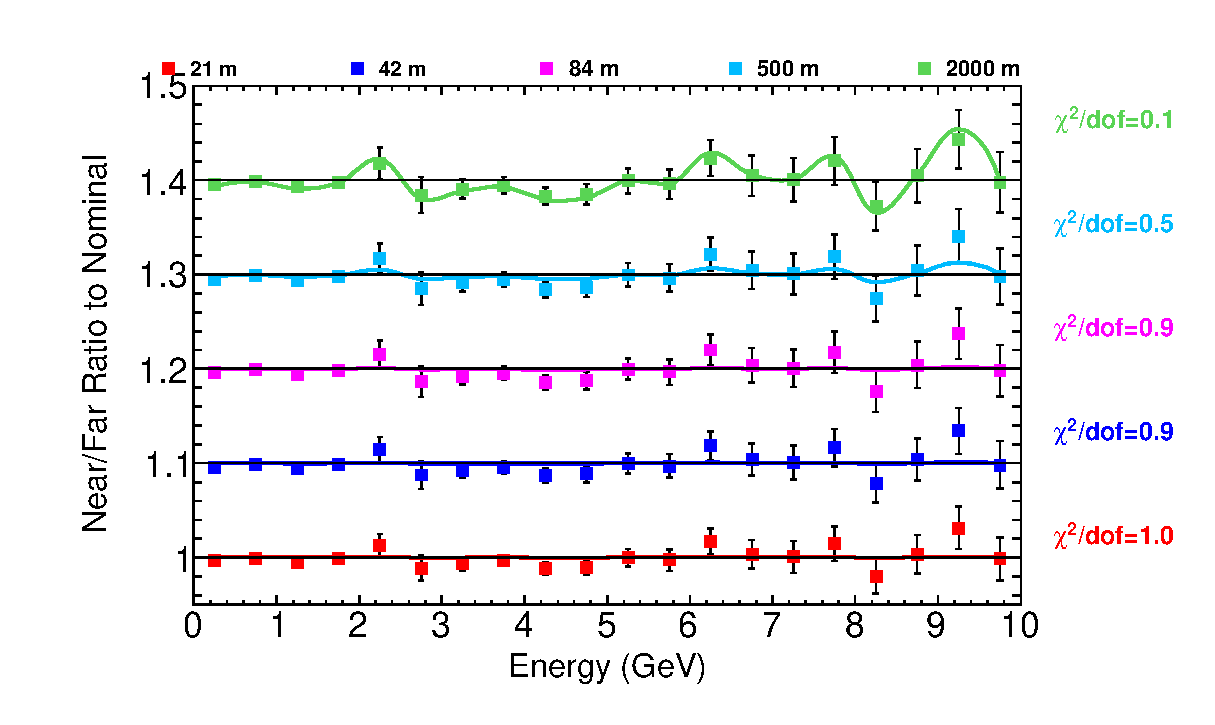
\includegraphics[width=6.0in]{figures/LBNEFDX_nof_summary.eps}}
  \end{center}
\caption{ Near/Far double ratios to nominal for several values of {\bf Far detector offset in $x$} (points) and the results of the fits to each energy bin (lines).}
\end{figure}

\begin{figure}[ht]
  \begin{center}
    {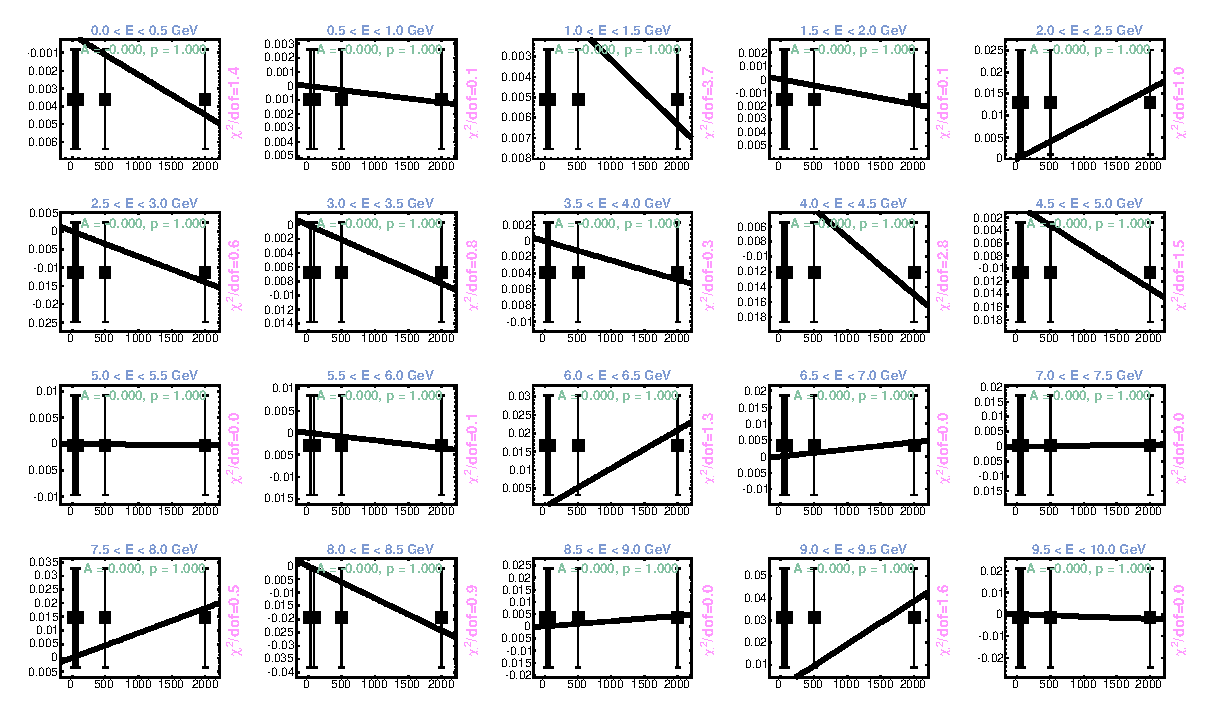
\includegraphics[width=5.0in]{figures/LBNEFDX_nof_fits.eps}}
  \end{center}
\caption{ Fits to the near/far ratios for several values of {\bf Far detector offset in $x$}. Black(Red) fit lines indicate that a linear(parabolic) fit provided the best $\chi^2$. }
\end{figure}

\begin{figure}[ht]
  \begin{center}
    {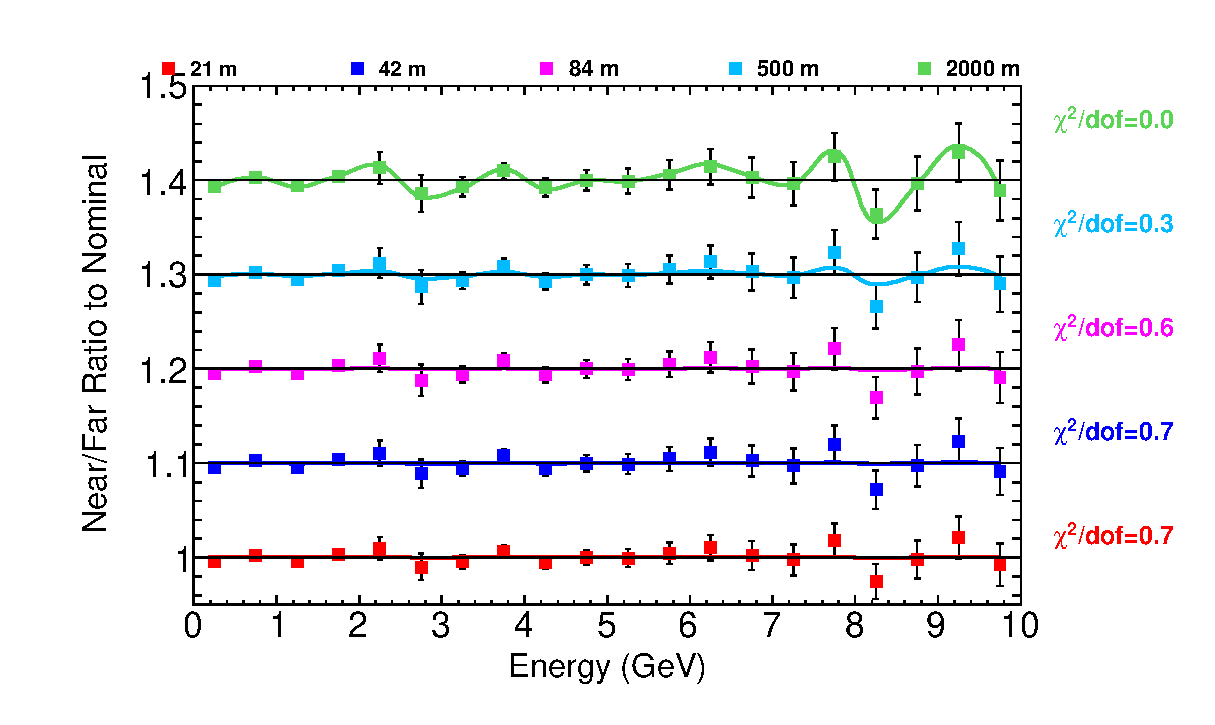
\includegraphics[width=6.0in]{figures/LBNEFDY_nof_summary.eps}}
  \end{center}
\caption{ Near/Far double ratios to nominal for several values of {\bf Far detector offset in $y$} (points) and the results of the fits to each energy bin (lines).}
\end{figure}

\begin{figure}[ht]
  \begin{center}
    {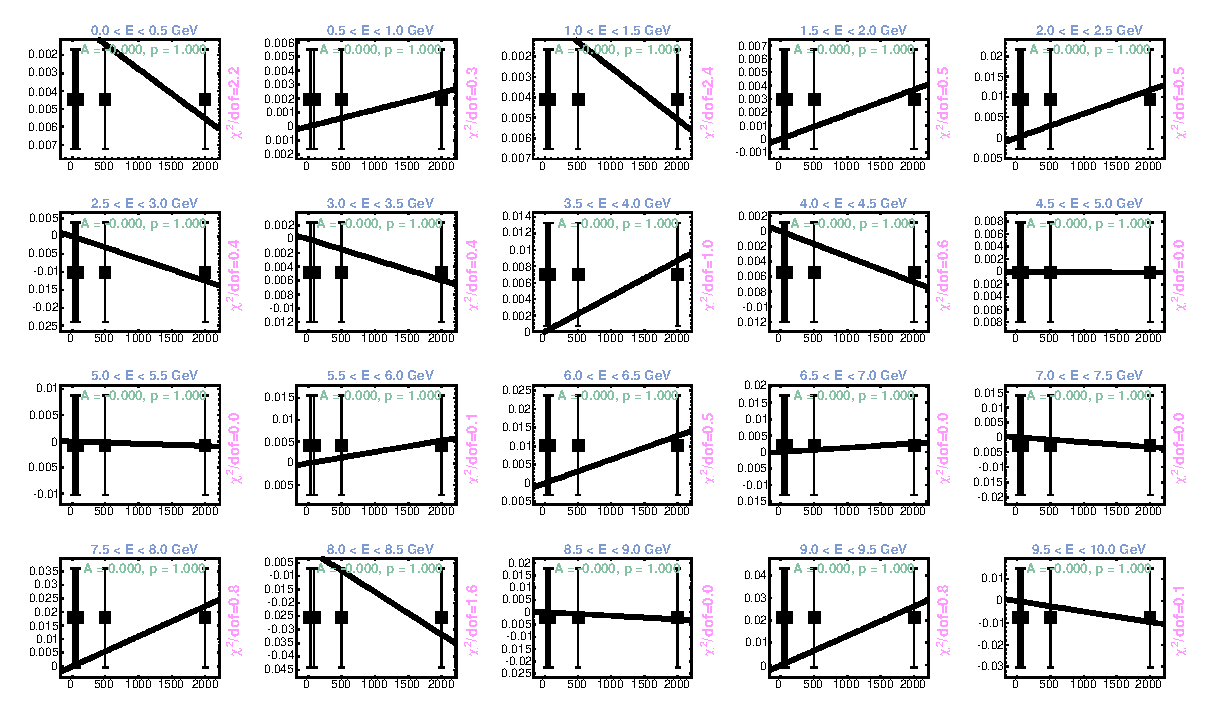
\includegraphics[width=5.0in]{figures/LBNEFDY_nof_fits.eps}}
  \end{center}
\caption{ Fits to the near/far ratios for several values of {\bf Far detector offset in $y$}. Black(Red) fit lines indicate that a linear(parabolic) fit provided the best $\chi^2$. }
\end{figure}

\begin{figure}[ht]
  \begin{center}
    {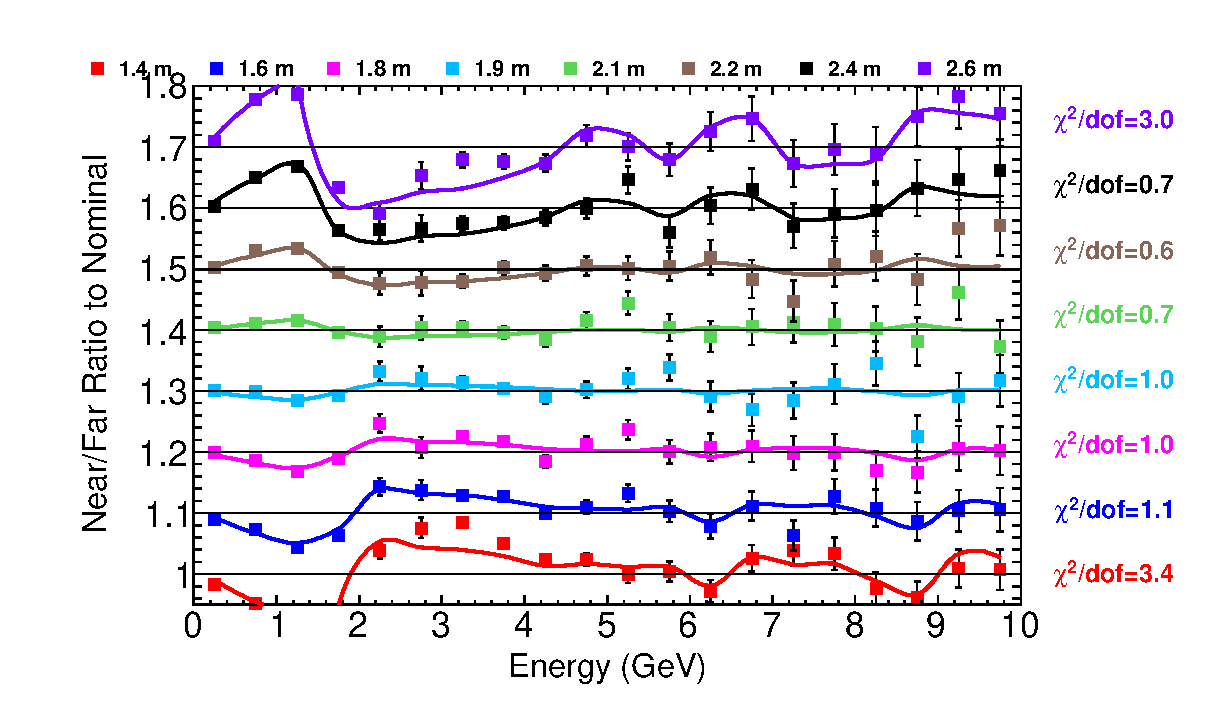
\includegraphics[width=6.0in]{figures/DecayPipeRadius_nof_summary.eps}}
  \end{center}
\caption{ Near/Far double ratios to nominal for several values of {\bf Decay Pipe Radius} (points) and the results of the fits to each energy bin (lines).}
\end{figure}

\begin{figure}[ht]
  \begin{center}
    {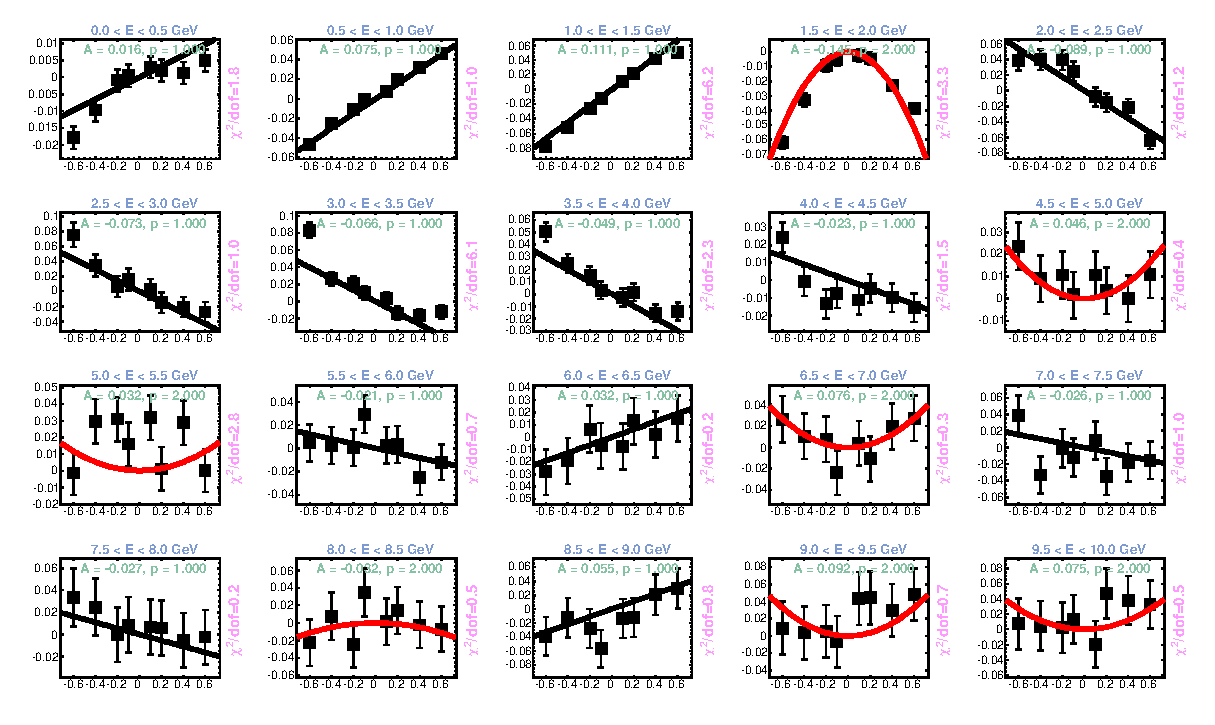
\includegraphics[width=5.0in]{figures/DecayPipeRadius_nof_fits.eps}}
  \end{center}
\caption{ Fits to the near/far ratios for several values of {\bf Decay Pipe Radius}. Black(Red) fit lines indicate that a linear(parabolic) fit provided the best $\chi^2$. }
\end{figure}

\begin{figure}[ht]
  \begin{center}
    {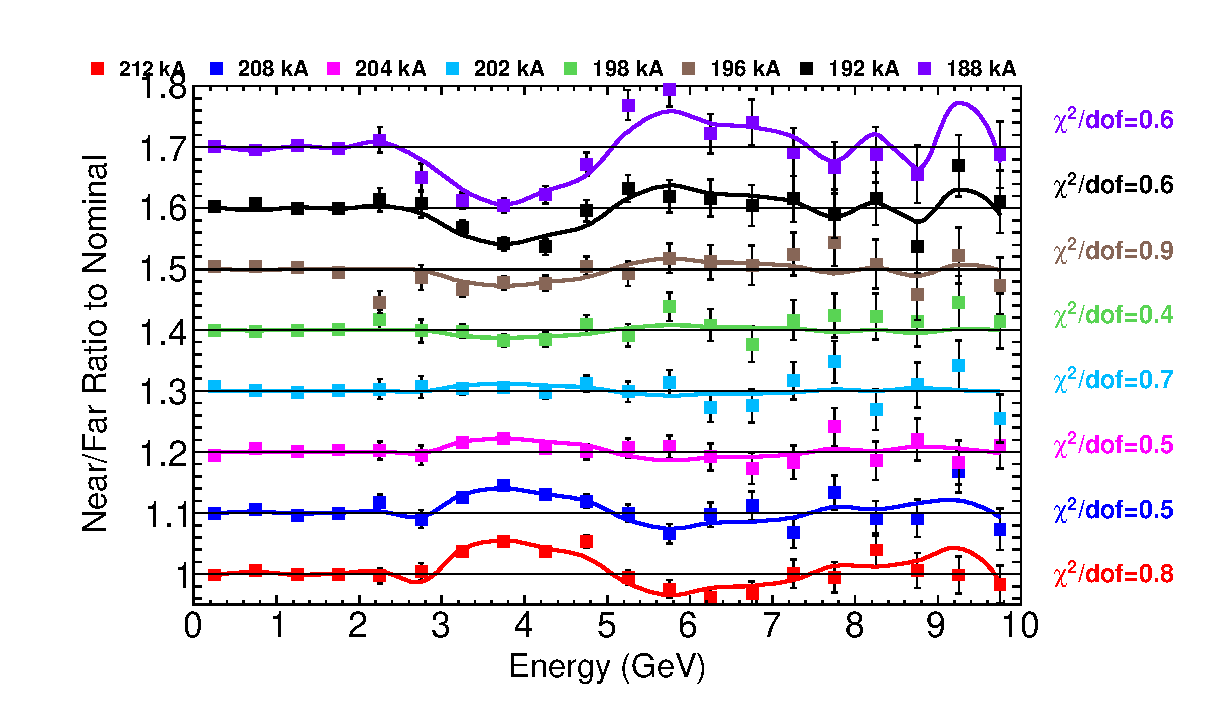
\includegraphics[width=6.0in]{figures/HornCurrent_nof_summary.eps}}
  \end{center}
\caption{ Near/Far double ratios to nominal for several values of {\bf Horn Current} (points) and the results of the fits to each energy bin (lines).}
\end{figure}

\begin{figure}[ht]
  \begin{center}
    {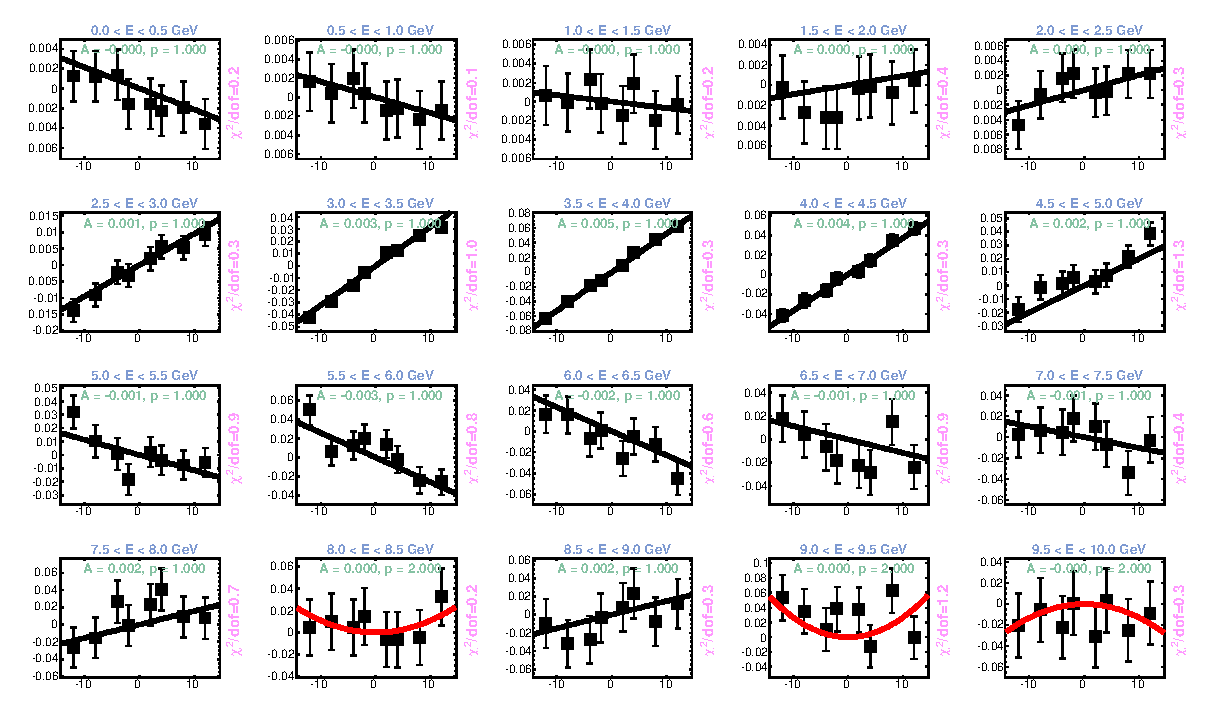
\includegraphics[width=5.0in]{figures/HornCurrent_nof_fits.eps}}
  \end{center}
\caption{ Fits to the near/far ratios for several values of {\bf HornCurrent}. Black(Red) fit lines indicate that a linear(parabolic) fit provided the best $\chi^2$. }
\end{figure}

\begin{figure}[ht]
  \begin{center}
    {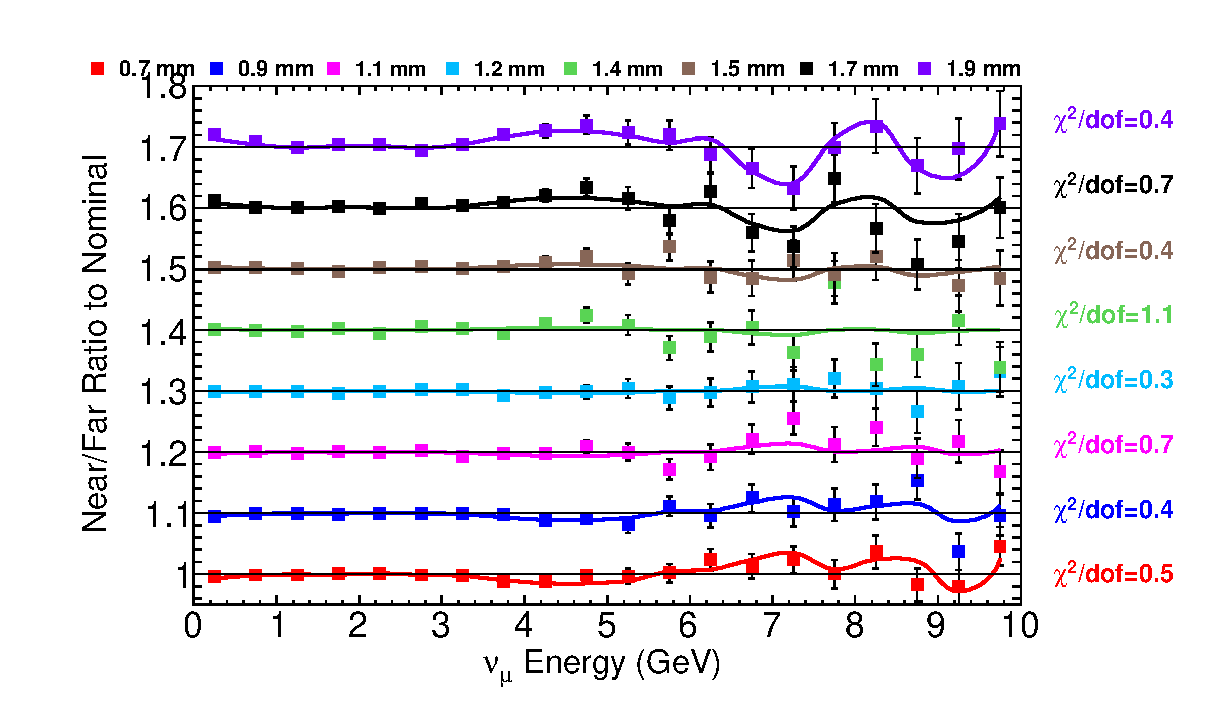
\includegraphics[width=6.0in]{figures/BeamSigmaX_nof_summary.eps}}
  \end{center}
\caption{ Near/Far double ratios to nominal for several values of {\bf Beam size in $x$} (points) and the results of the fits to each energy bin (lines).}
\end{figure}

\begin{figure}[ht]
  \begin{center}
    {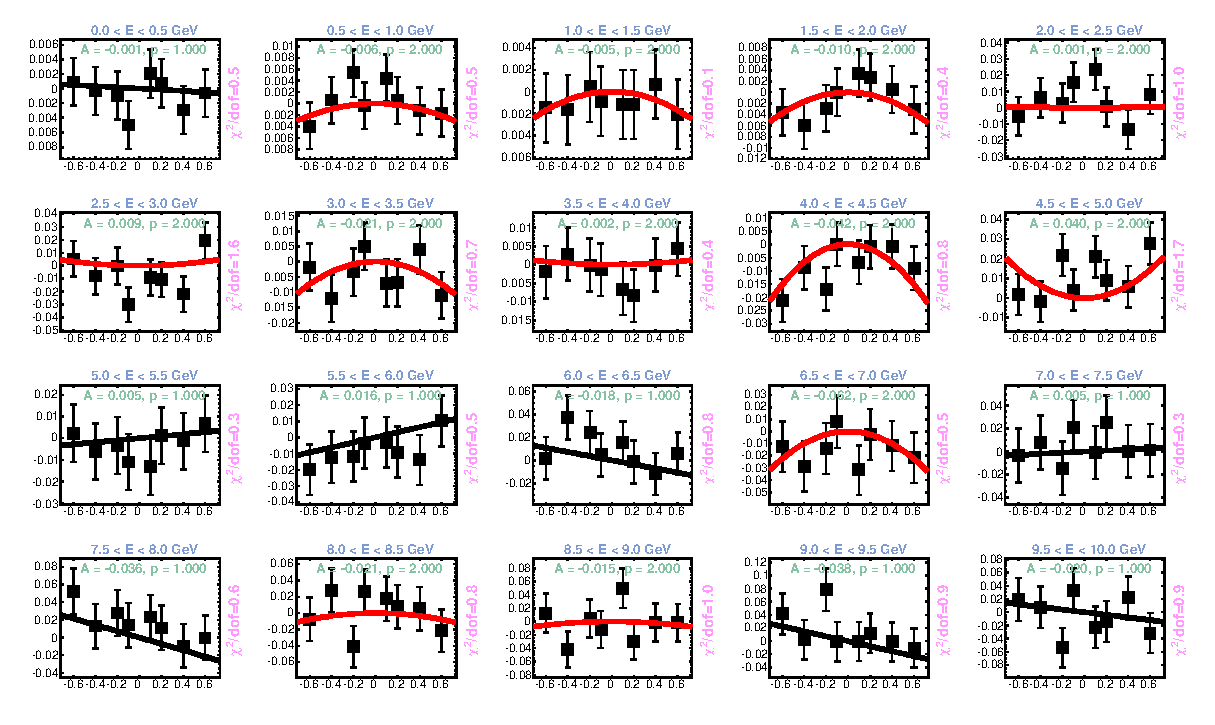
\includegraphics[width=5.0in]{figures/BeamSigmaY_nof_fits.eps}}
  \end{center}
\caption{ Fits to the near/far ratios for several values of {\bf Beam size in $y$}. Black(Red) fit lines indicate that a linear(parabolic) fit provided the best $\chi^2$. }
\end{figure}

\clearpage

\begin{figure}[ht]
  \begin{center}
    {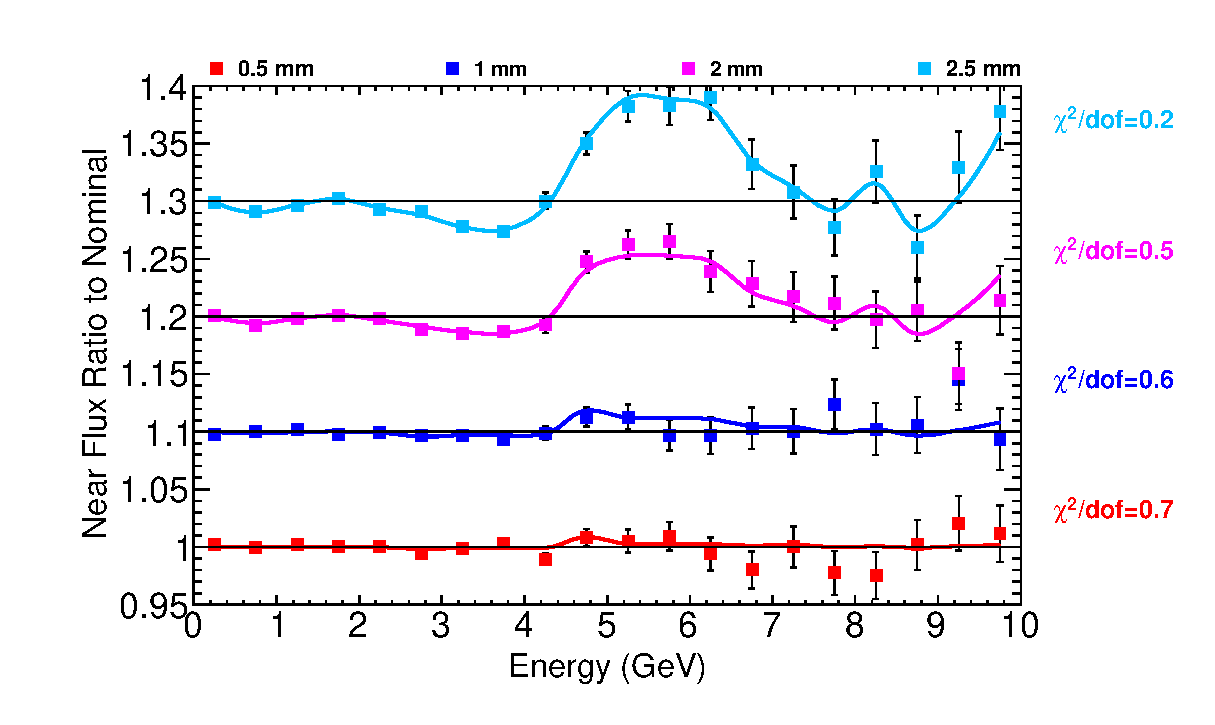
\includegraphics[width=6.0in]{figures/Horn1XOffset_near_summary.eps}}
  \end{center}
\caption{ Near detector flux ratios to nominal for several values of {\bf Horn 1 Offset in $x$} (points) and the results of the fits to each energy bin (lines).}
\end{figure}

\begin{figure}[ht]
  \begin{center}
    {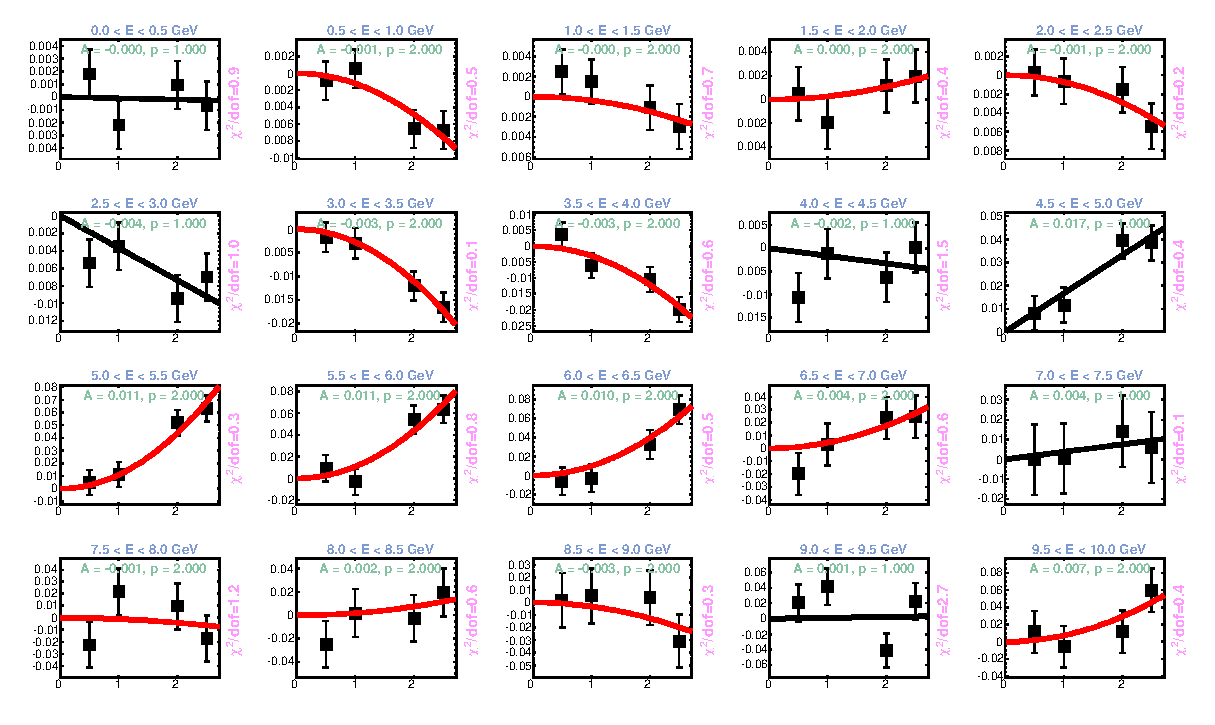
\includegraphics[width=5.0in]{figures/Horn1XOffset_near_fits.eps}}
  \end{center}
\caption{ Fits to the far flux ratios for several values of {\bf Horn 1 Offset in $x$}. Black(Red) fit lines indicate that a linear(parabolic) fit provided the best $\chi^2$. }
\end{figure}

\begin{figure}[ht]
  \begin{center}
    {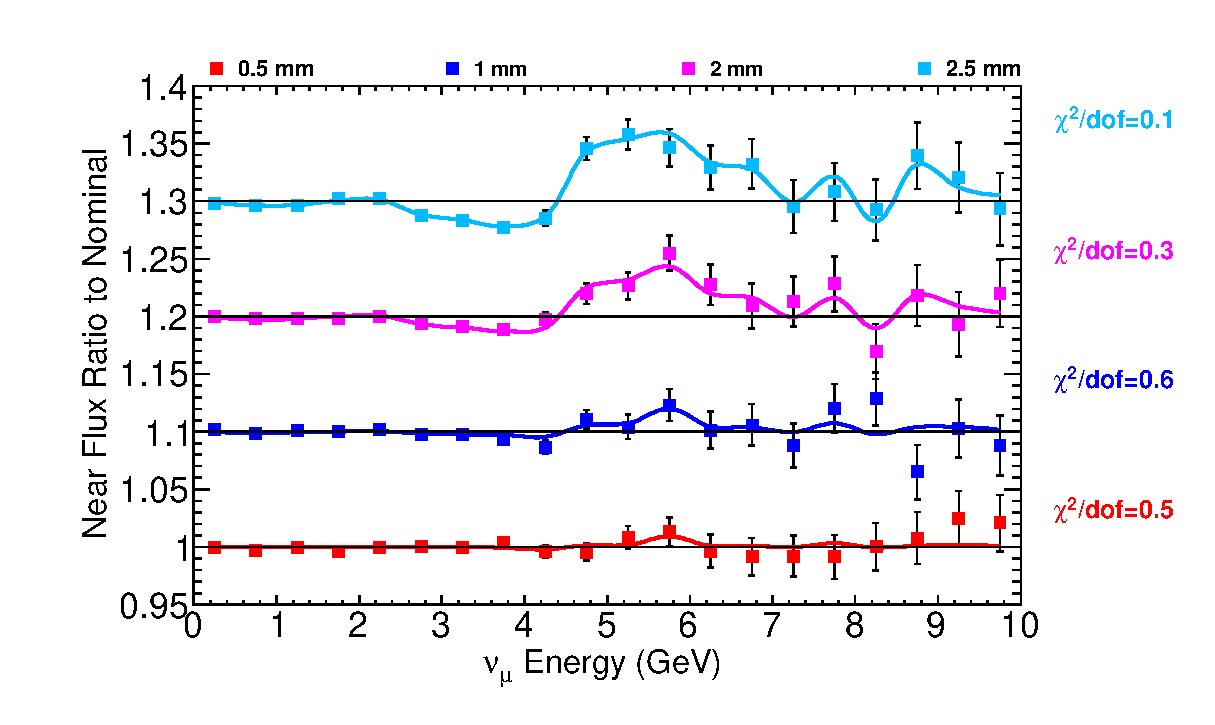
\includegraphics[width=6.0in]{figures/Horn1YOffset_near_summary.eps}}
  \end{center}
\caption{ Near detector flux ratios to nominal for several values of {\bf Horn 1 Offset in $y$} (points) and the results of the fits to each energy bin (lines).}
\end{figure}

\begin{figure}[ht]
  \begin{center}
    {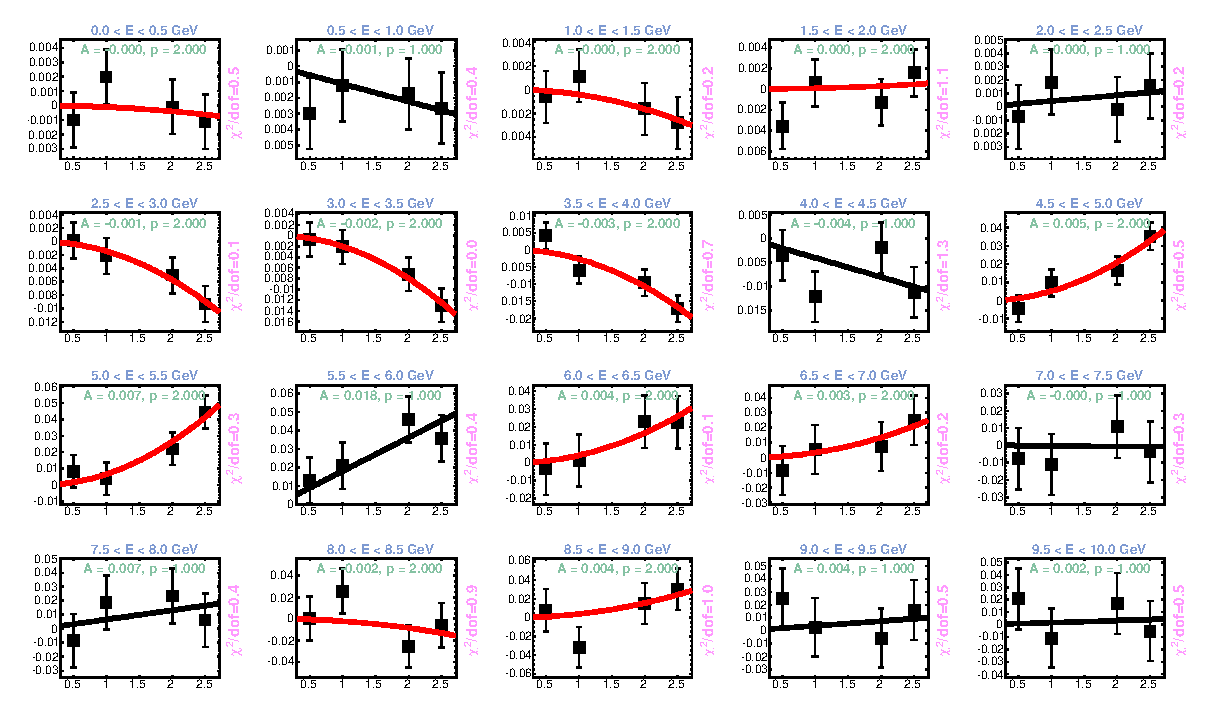
\includegraphics[width=5.0in]{figures/Horn1YOffset_near_fits.eps}}
  \end{center}
\caption{ Fits to the near flux ratios for several values of {\bf Horn 1 Offset in $y$}. Black(Red) fit lines indicate that a linear(parabolic) fit provided the best $\chi^2$. }
\end{figure}

\begin{figure}[ht]
  \begin{center}
    {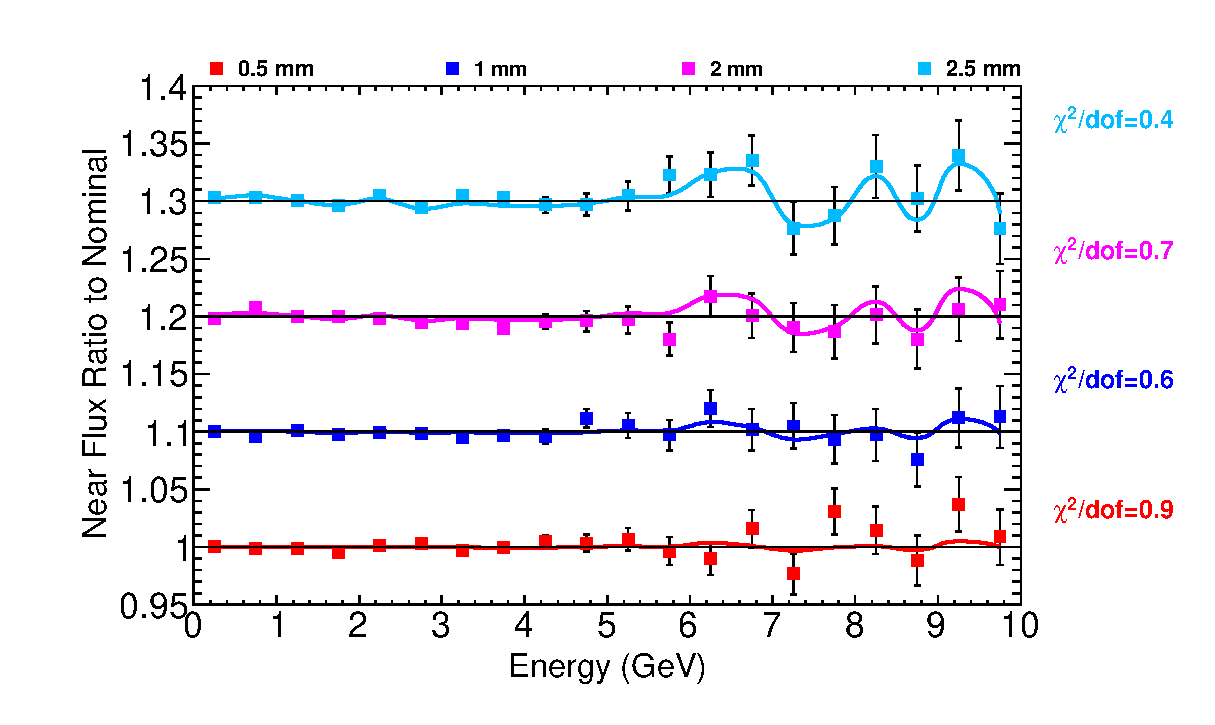
\includegraphics[width=6.0in]{figures/Horn2XOffset_near_summary.eps}}
  \end{center}
\caption{ Near detector flux ratios to nominal for several values of {\bf Horn 2 Offset in $x$} (points) and the results of the fits to each energy bin (lines).}
\end{figure}

\begin{figure}[ht]
  \begin{center}
    {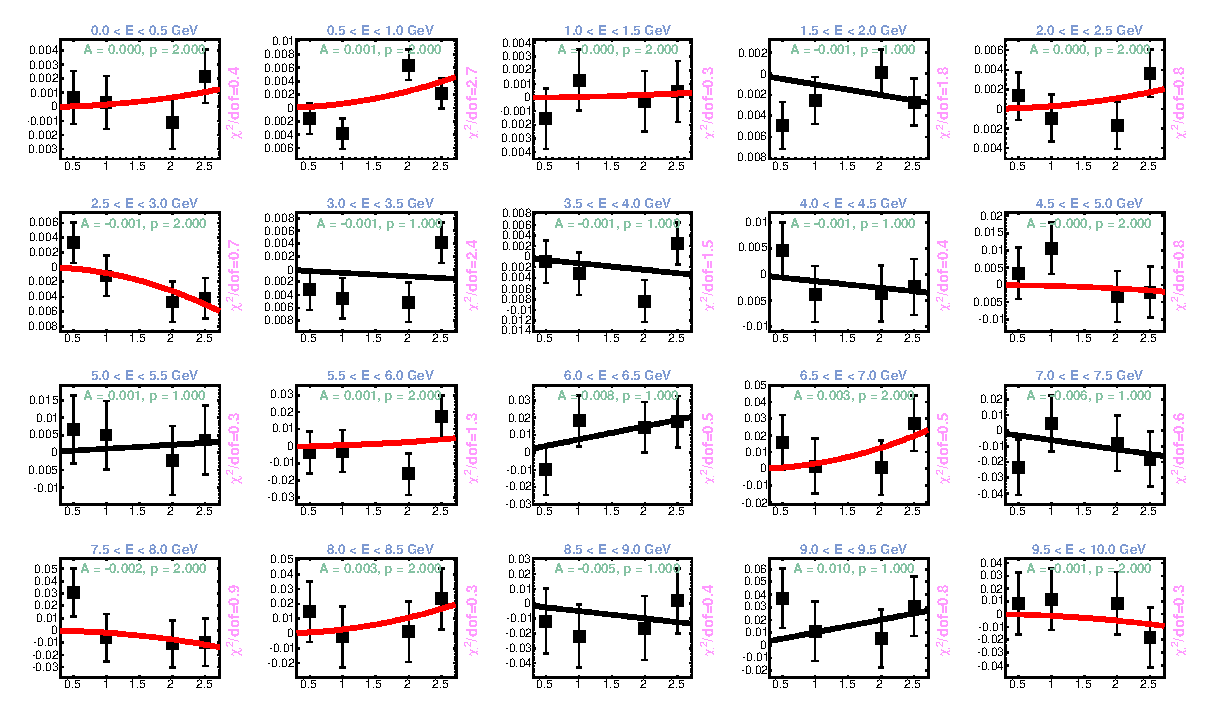
\includegraphics[width=5.0in]{figures/Horn2XOffset_near_fits.eps}}
  \end{center}
\caption{ Fits to the near flux ratios for several values of {\bf Horn 2 Offset in $x$}. Black(Red) fit lines indicate that a linear(parabolic) fit provided the best $\chi^2$. }
\end{figure}

\begin{figure}[ht]
  \begin{center}
    {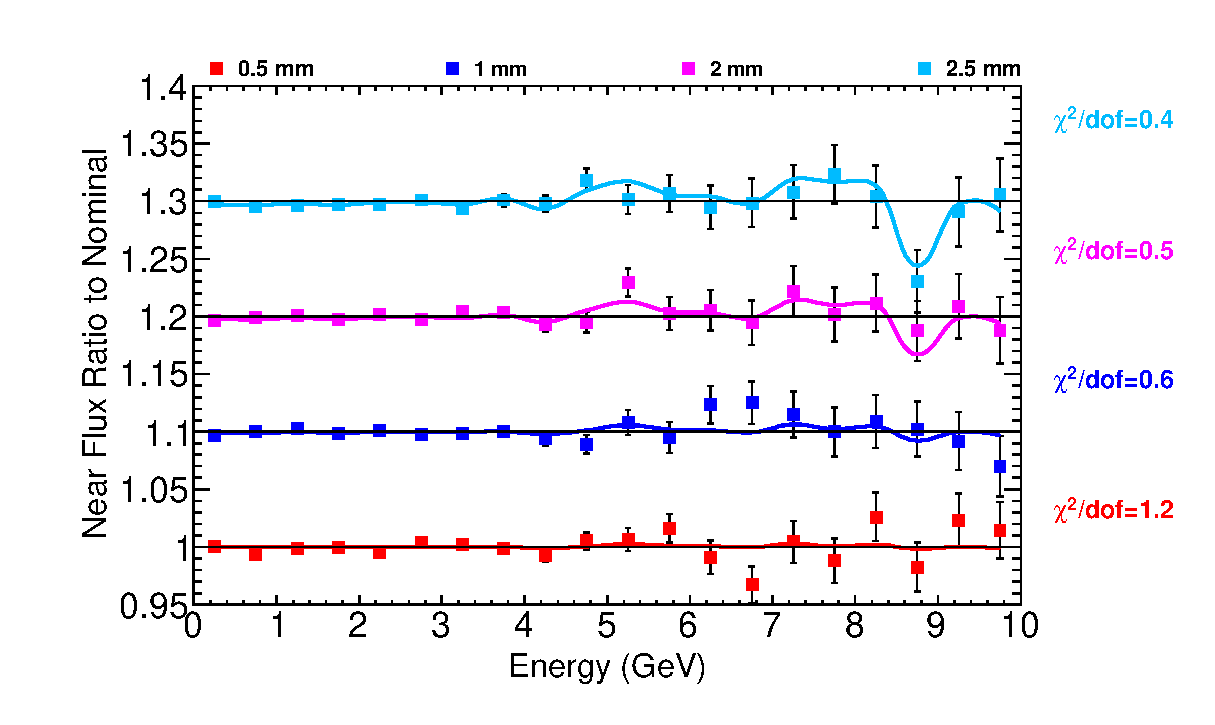
\includegraphics[width=6.0in]{figures/Horn2YOffset_near_summary.eps}}
  \end{center}
\caption{ Near detector flux ratios to nominal for several values of {\bf Horn 2 Offset in $y$} (points) and the results of the fits to each energy bin (lines).}
\end{figure}

\begin{figure}[ht]
  \begin{center}
    {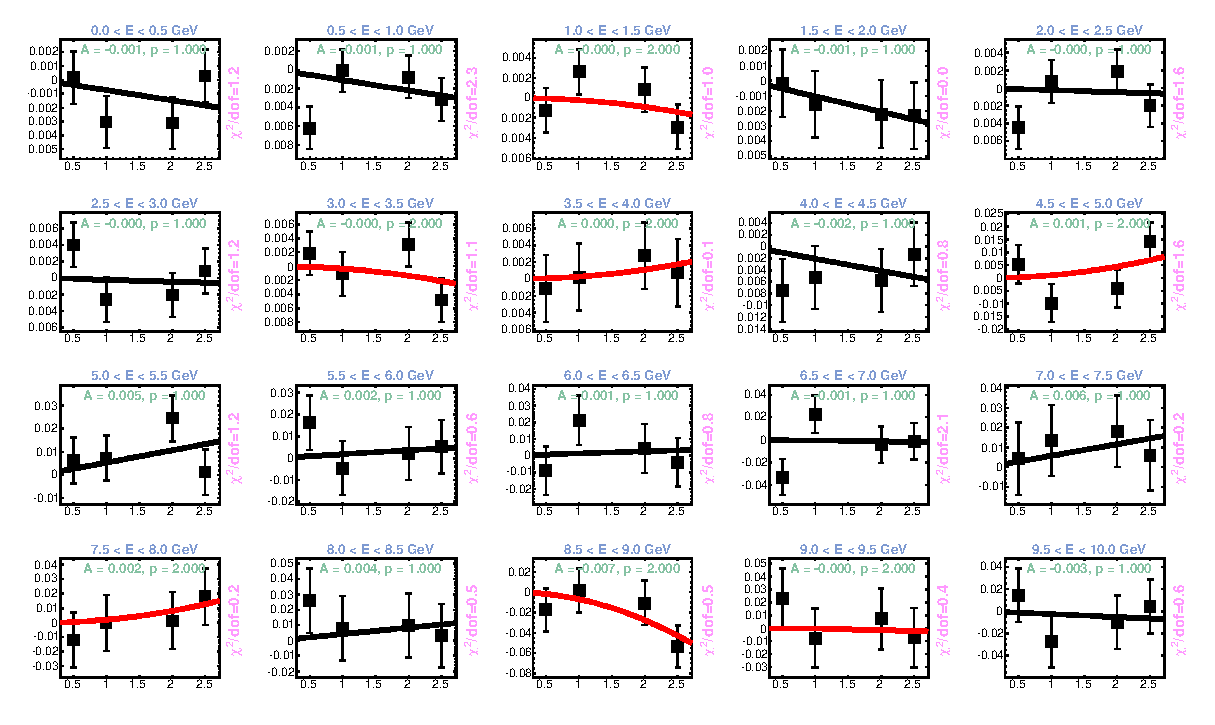
\includegraphics[width=5.0in]{figures/Horn2YOffset_near_fits.eps}}
  \end{center}
\caption{ Fits to the near flux ratios for several values of {\bf Horn 2 Offset in $y$}. Black(Red) fit lines indicate that a linear(parabolic) fit provided the best $\chi^2$. }
\end{figure}

\begin{figure}[ht]
  \begin{center}
    {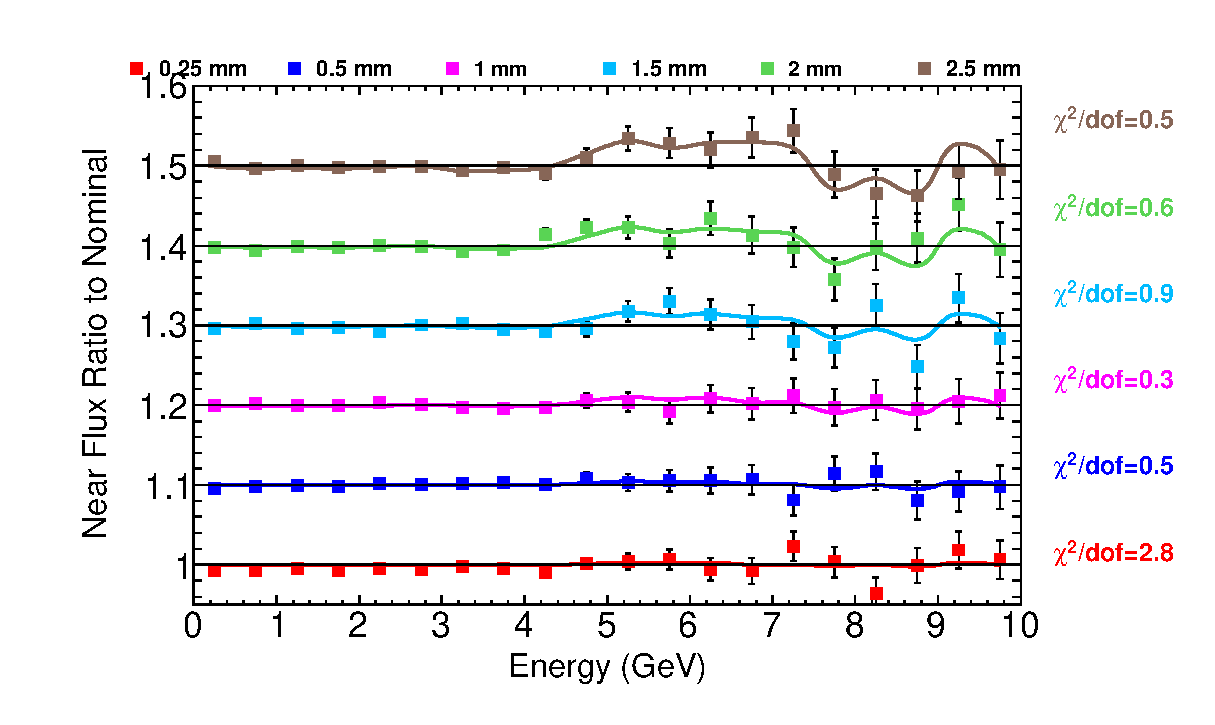
\includegraphics[width=6.0in]{figures/Horn1XTilt_near_summary.eps}}
  \end{center}
\caption{ Near detector flux ratios to nominal for several values of {\bf Horn 1 Tilt in $x$} (points) and the results of the fits to each energy bin (lines).}
\end{figure}

\begin{figure}[ht]
  \begin{center}
    {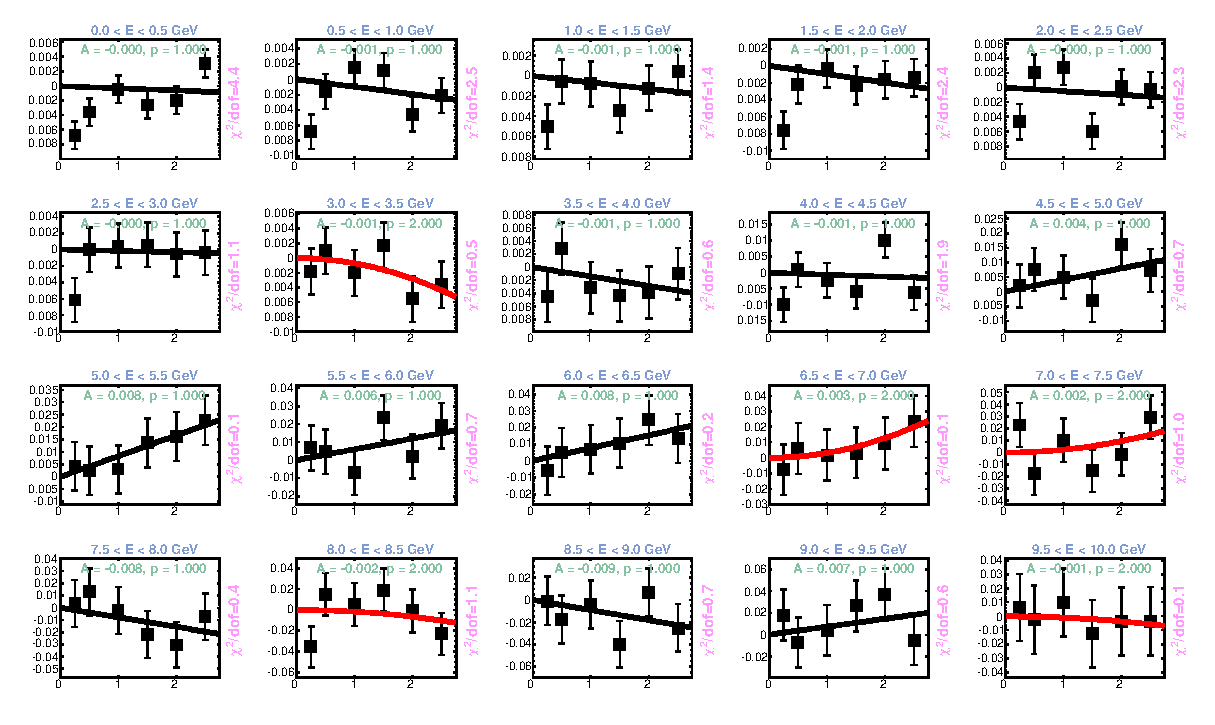
\includegraphics[width=5.0in]{figures/Horn1XTilt_near_fits.eps}}
  \end{center}
\caption{ Fits to the near flux ratios for several values of {\bf Horn 1 Tilt in $x$}. Black(Red) fit lines indicate that a linear(parabolic) fit provided the best $\chi^2$. }
\end{figure}

\begin{figure}[ht]
  \begin{center}
    {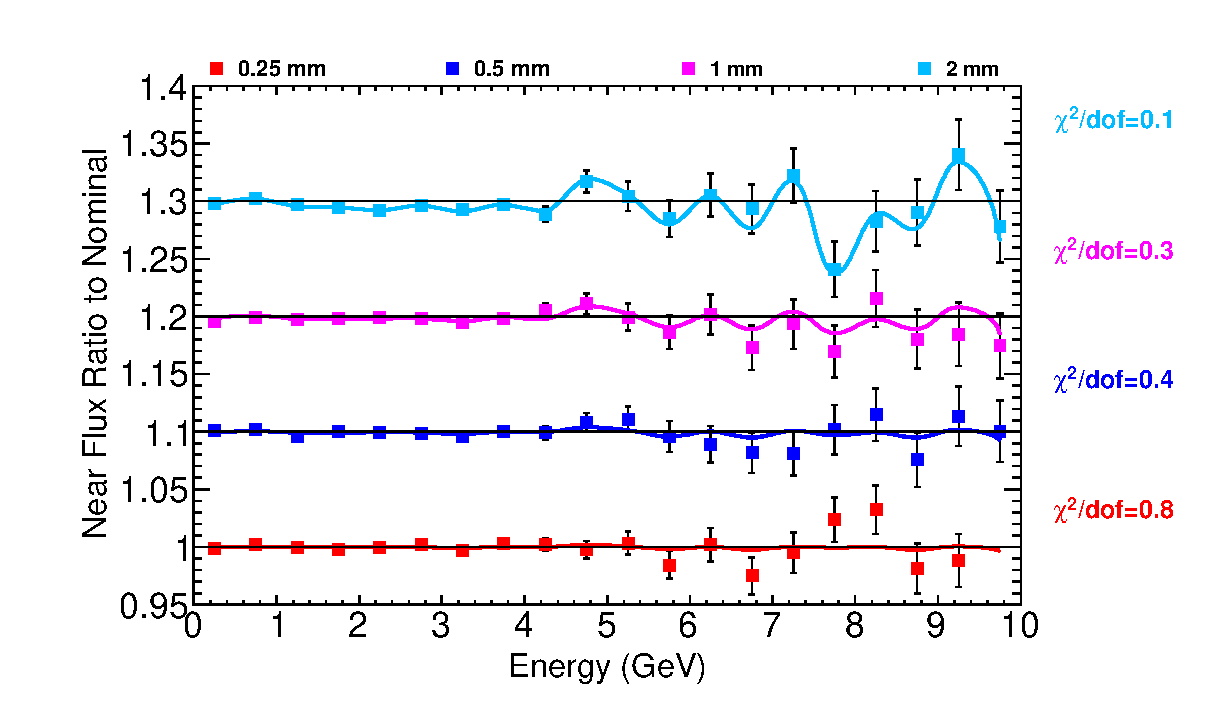
\includegraphics[width=6.0in]{figures/Horn1YTilt_near_summary.eps}}
  \end{center}
\caption{ Near detector flux ratios to nominal for several values of {\bf Horn 1 Tilt in $y$} (points) and the results of the fits to each energy bin (lines).}
\end{figure}

\begin{figure}[ht]
  \begin{center}
    {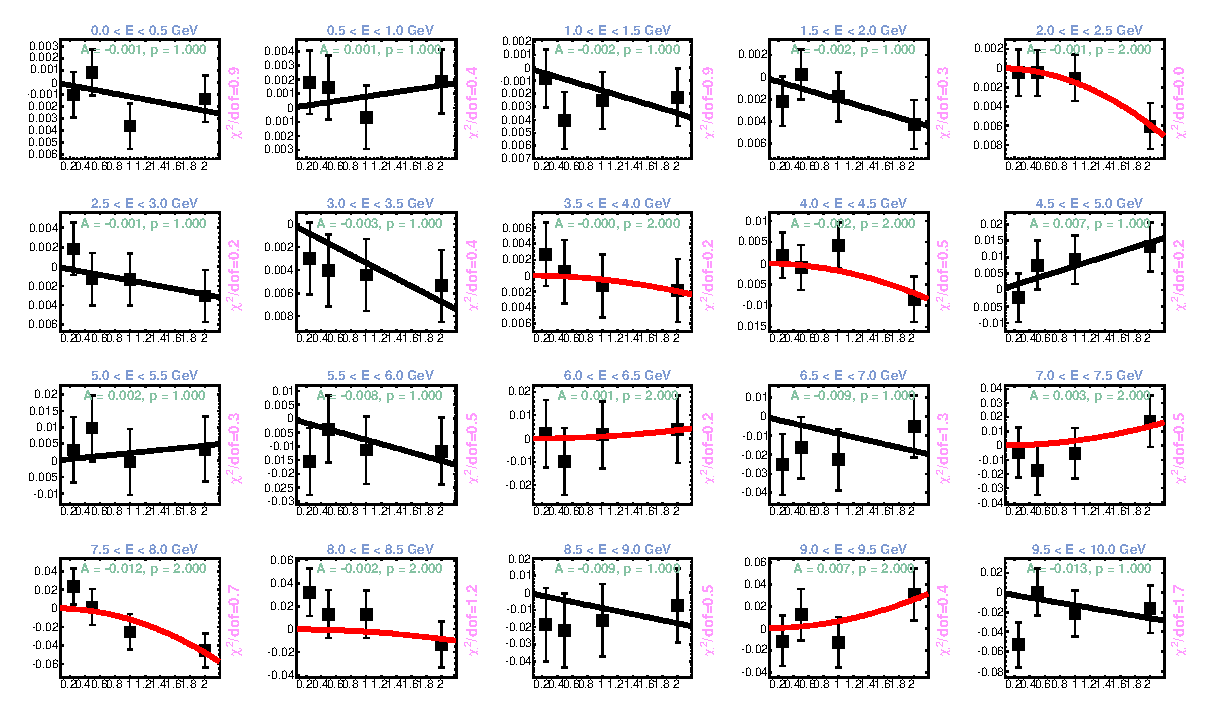
\includegraphics[width=5.0in]{figures/Horn1YTilt_near_fits.eps}}
  \end{center}
\caption{ Fits to the near flux ratios for several values of {\bf Horn 1 Tilt in $y$}. Black(Red) fit lines indicate that a linear(parabolic) fit provided the best $\chi^2$. }
\end{figure}

\clearpage

\begin{figure}[ht]
  \begin{center}
    {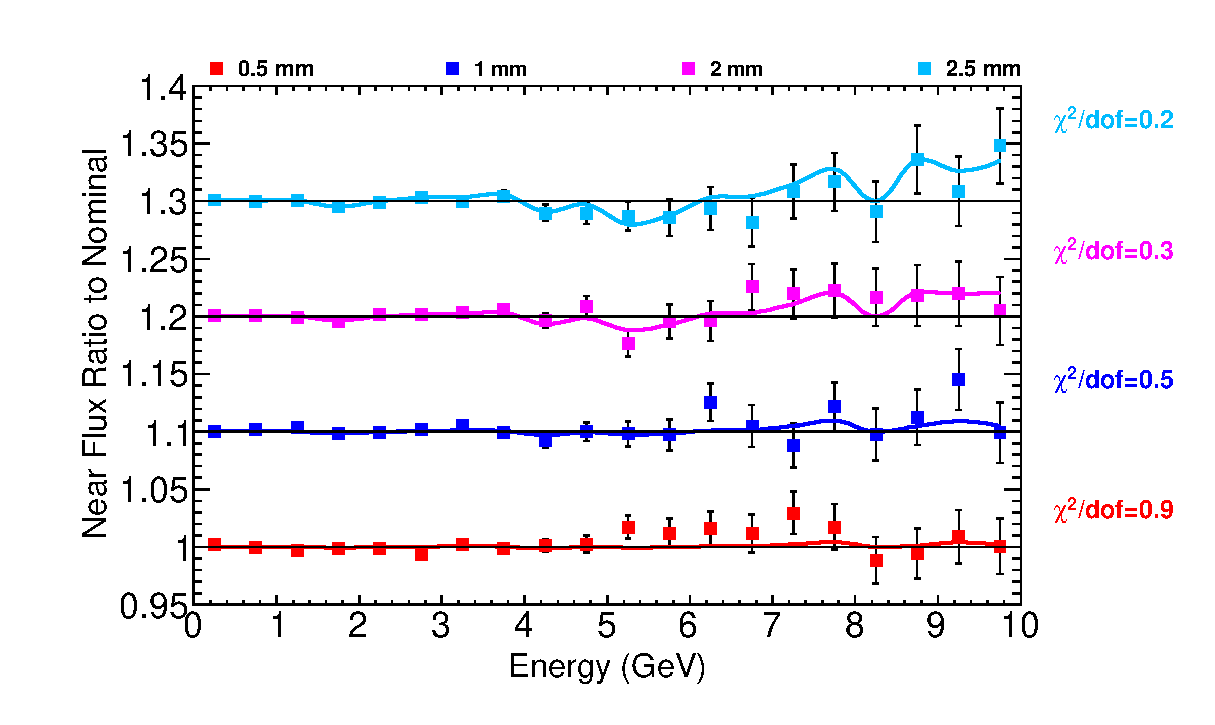
\includegraphics[width=6.0in]{figures/Horn2XTilt_near_summary.eps}}
  \end{center}
\caption{ Near detector flux ratios to nominal for several values of {\bf Horn 2 Tilt in $x$} (points) and the results of the fits to each energy bin (lines).}
\end{figure}

\begin{figure}[ht]
  \begin{center}
    {\includegraphics[width=5.0in]{figures/Horn2XTilt_near_fits.eps}}
  \end{center}
\caption{ Fits to the near flux ratios for several values of {\bf Horn 2 Tilt in $x$}. Black(Red) fit lines indicate that a linear(parabolic) fit provided the best $\chi^2$. }
\end{figure}

\begin{figure}[ht]
  \begin{center}
    {\includegraphics[width=6.0in]{figures/Horn2YTilt_near_summary.eps}}
  \end{center}
\caption{ Near detector flux ratios to nominal for several values of {\bf Horn 2 Tilt in $y$} (points) and the results of the fits to each energy bin (lines).}
\end{figure}

\begin{figure}[ht]
  \begin{center}
    {\includegraphics[width=5.0in]{figures/Horn2YTilt_near_fits.eps}}
  \end{center}
\caption{ Fits to the near flux ratios for several values of {\bf Horn 2 Tilt in $y$}. Black(Red) fit lines indicate that a linear(parabolic) fit provided the best $\chi^2$. }
\end{figure}

\begin{figure}[ht]
  \begin{center}
    {\includegraphics[width=6.0in]{figures/TargetXOffset_near_summary.eps}}
  \end{center}
\caption{ Near detector flux ratios to nominal for several values of {\bf Target Offset in $x$} (points) and the results of the fits to each energy bin (lines).}
\end{figure}

\begin{figure}[ht]
  \begin{center}
    {\includegraphics[width=5.0in]{figures/TargetXOffset_near_fits.eps}}
  \end{center}
\caption{ Fits to the near flux ratios for several values of {\bf Target Offset in $x$}. Black(Red) fit lines indicate that a linear(parabolic) fit provided the best $\chi^2$. }
\end{figure}

\begin{figure}[ht]
  \begin{center}
    {\includegraphics[width=6.0in]{figures/TargetYOffset_near_summary.eps}}
  \end{center}
\caption{ Near detector flux ratios to nominal for several values of {\bf Target Offset in $y$} (points) and the results of the fits to each energy bin (lines).}
\end{figure}

\begin{figure}[ht]
  \begin{center}
    {\includegraphics[width=5.0in]{figures/TargetYOffset_near_fits.eps}}
  \end{center}
\caption{ Fits to the near flux ratios for several values of {\bf Target Offset in $y$}. Black(Red) fit lines indicate that a linear(parabolic) fit provided the best $\chi^2$. }
\end{figure}

\begin{figure}[ht]
  \begin{center}
    {\includegraphics[width=6.0in]{figures/TargetXTilt_near_summary.eps}}
  \end{center}
\caption{ Near detector flux ratios to nominal for several values of {\bf Target Tilt in $x$} (points) and the results of the fits to each energy bin (lines).}
\end{figure}

\begin{figure}[ht]
  \begin{center}
    {\includegraphics[width=5.0in]{figures/TargetXTilt_near_fits.eps}}
  \end{center}
\caption{ Fits to the near flux ratios for several values of {\bf Target Tilt in $x$}. Black(Red) fit lines indicate that a linear(parabolic) fit provided the best $\chi^2$. }
\end{figure}

\clearpage

\begin{figure}[ht]
  \begin{center}
    {\includegraphics[width=6.0in]{figures/TargetYTilt_near_summary.eps}}
  \end{center}
\caption{ Near detector flux ratios to nominal for several values of {\bf Target Tilt in $y$} (points) and the results of the fits to each energy bin (lines).}
\end{figure}

\begin{figure}[ht]
  \begin{center}
    {\includegraphics[width=5.0in]{figures/TargetYTilt_near_fits.eps}}
  \end{center}
\caption{ Fits to the near flux ratios for several values of {\bf Target Tilt in $y$}. Black(Red) fit lines indicate that a linear(parabolic) fit provided the best $\chi^2$. }
\end{figure}


\begin{figure}[ht]
  \begin{center}
    {\includegraphics[width=6.0in]{figures/LBNEFDX_near_summary.eps}}
  \end{center}
\caption{ Near detector flux ratios to nominal for several values of {\bf Far detector offset in $x$} (points) and the results of the fits to each energy bin (lines).}
\end{figure}

\begin{figure}[ht]
  \begin{center}
    {\includegraphics[width=5.0in]{figures/LBNEFDX_near_fits.eps}}
  \end{center}
\caption{ Fits to the near flux ratios for several values of {\bf Far detector offset in $x$}. Black(Red) fit lines indicate that a linear(parabolic) fit provided the best $\chi^2$. }
\end{figure}

\begin{figure}[ht]
  \begin{center}
    {\includegraphics[width=6.0in]{figures/LBNEFDY_near_summary.eps}}
  \end{center}
\caption{ Near detector flux ratios to nominal for several values of {\bf Near detector offset in $y$} (points) and the results of the fits to each energy bin (lines).}
\end{figure}

\begin{figure}[ht]
  \begin{center}
    {\includegraphics[width=5.0in]{figures/LBNEFDY_near_fits.eps}}
  \end{center}
\caption{ Fits to the near flux ratios for several values of {\bf Near detector offset in $y$}. Black(Red) fit lines indicate that a linear(parabolic) fit provided the best $\chi^2$. }
\end{figure}

\begin{figure}[ht]
  \begin{center}
    {\includegraphics[width=6.0in]{figures/DecayPipeRadius_near_summary.eps}}
  \end{center}
\caption{ Near detector flux ratios to nominal for several values of {\bf Decay Pipe Radius} (points) and the results of the fits to each energy bin (lines).}
\end{figure}

\begin{figure}[ht]
  \begin{center}
    {\includegraphics[width=5.0in]{figures/DecayPipeRadius_near_fits.eps}}
  \end{center}
\caption{ Fits to the near flux ratios for several values of {\bf Decay Pipe Radius}. Black(Red) fit lines indicate that a linear(parabolic) fit provided the best $\chi^2$. }
\end{figure}

\begin{figure}[ht]
  \begin{center}
    {\includegraphics[width=6.0in]{figures/HornCurrent_near_summary.eps}}
  \end{center}
\caption{ Near detector flux ratios to nominal for several values of {\bf Horn Current} (points) and the results of the fits to each energy bin (lines).}
\end{figure}

\begin{figure}[ht]
  \begin{center}
    {\includegraphics[width=5.0in]{figures/HornCurrent_near_fits.eps}}
  \end{center}
\caption{ Fits to the near flux ratios for several values of {\bf HornCurrent}. Black(Red) fit lines indicate that a linear(parabolic) fit provided the best $\chi^2$. }
\end{figure}

\begin{figure}[ht]
  \begin{center}
    {\includegraphics[width=6.0in]{figures/BeamSigmaX_near_summary.eps}}
  \end{center}
\caption{ Near detector flux ratios to nominal for several values of {\bf Beam size in $x$} (points) and the results of the fits to each energy bin (lines).}
\end{figure}

\begin{figure}[ht]
  \begin{center}
    {\includegraphics[width=5.0in]{figures/BeamSigmaY_near_fits.eps}}
  \end{center}
\caption{ Fits to the near flux ratios for several values of {\bf Beam size in $y$}. Black(Red) fit lines indicate that a linear(parabolic) fit provided the best $\chi^2$. }
\end{figure}

\clearpage

\begin{figure}[ht]
  \begin{center}
    {\includegraphics[width=6.0in]{figures/Horn1XOffset_far_summary.eps}}
  \end{center}
\caption{ Far detector flux ratios to nominal for several values of {\bf Horn 1 Offset in $x$} (points) and the results of the fits to each energy bin (lines).}
\end{figure}

\begin{figure}[ht]
  \begin{center}
    {\includegraphics[width=5.0in]{figures/Horn1XOffset_far_fits.eps}}
  \end{center}
\caption{ Fits to the far flux ratios for several values of {\bf Horn 1 Offset in $x$}. Black(Red) fit lines indicate that a linear(parabolic) fit provided the best $\chi^2$. }
\end{figure}

\begin{figure}[ht]
  \begin{center}
    {\includegraphics[width=6.0in]{figures/Horn1YOffset_far_summary.eps}}
  \end{center}
\caption{ Far detector flux ratios to nominal for several values of {\bf Horn 1 Offset in $y$} (points) and the results of the fits to each energy bin (lines).}
\end{figure}

\begin{figure}[ht]
  \begin{center}
    {\includegraphics[width=5.0in]{figures/Horn1YOffset_far_fits.eps}}
  \end{center}
\caption{ Fits to the far flux ratios for several values of {\bf Horn 1 Offset in $y$}. Black(Red) fit lines indicate that a linear(parabolic) fit provided the best $\chi^2$. }
\end{figure}

\begin{figure}[ht]
  \begin{center}
    {\includegraphics[width=6.0in]{figures/Horn2XOffset_far_summary.eps}}
  \end{center}
\caption{ Far detector flux ratios to nominal for several values of {\bf Horn 2 Offset in $x$} (points) and the results of the fits to each energy bin (lines).}
\end{figure}

\begin{figure}[ht]
  \begin{center}
    {\includegraphics[width=5.0in]{figures/Horn2XOffset_far_fits.eps}}
  \end{center}
\caption{ Fits to the far flux ratios for several values of {\bf Horn 2 Offset in $x$}. Black(Red) fit lines indicate that a linear(parabolic) fit provided the best $\chi^2$. }
\end{figure}

\begin{figure}[ht]
  \begin{center}
    {\includegraphics[width=6.0in]{figures/Horn2YOffset_far_summary.eps}}
  \end{center}
\caption{ Far detector flux ratios to nominal for several values of {\bf Horn 2 Offset in $y$} (points) and the results of the fits to each energy bin (lines).}
\end{figure}

\begin{figure}[ht]
  \begin{center}
    {\includegraphics[width=5.0in]{figures/Horn2YOffset_far_fits.eps}}
  \end{center}
\caption{ Fits to the far flux ratios for several values of {\bf Horn 2 Offset in $y$}. Black(Red) fit lines indicate that a linear(parabolic) fit provided the best $\chi^2$. }
\end{figure}

\begin{figure}[ht]
  \begin{center}
    {\includegraphics[width=6.0in]{figures/Horn1XTilt_far_summary.eps}}
  \end{center}
\caption{ Far detector flux ratios to nominal for several values of {\bf Horn 1 Tilt in $x$} (points) and the results of the fits to each energy bin (lines).}
\end{figure}

\begin{figure}[ht]
  \begin{center}
    {\includegraphics[width=5.0in]{figures/Horn1XTilt_far_fits.eps}}
  \end{center}
\caption{ Fits to the far flux ratios for several values of {\bf Horn 1 Tilt in $x$}. Black(Red) fit lines indicate that a linear(parabolic) fit provided the best $\chi^2$. }
\end{figure}

\begin{figure}[ht]
  \begin{center}
    {\includegraphics[width=6.0in]{figures/Horn1YTilt_far_summary.eps}}
  \end{center}
\caption{ Far detector flux ratios to nominal for several values of {\bf Horn 1 Tilt in $y$} (points) and the results of the fits to each energy bin (lines).}
\end{figure}

\begin{figure}[ht]
  \begin{center}
    {\includegraphics[width=5.0in]{figures/Horn1YTilt_far_fits.eps}}
  \end{center}
\caption{ Fits to the far flux ratios for several values of {\bf Horn 1 Tilt in $y$}. Black(Red) fit lines indicate that a linear(parabolic) fit provided the best $\chi^2$. }
\end{figure}

\clearpage

\begin{figure}[ht]
  \begin{center}
    {\includegraphics[width=6.0in]{figures/Horn2XTilt_far_summary.eps}}
  \end{center}
\caption{ Far detector flux ratios to nominal for several values of {\bf Horn 2 Tilt in $x$} (points) and the results of the fits to each energy bin (lines).}
\end{figure}

\begin{figure}[ht]
  \begin{center}
    {\includegraphics[width=5.0in]{figures/Horn2XTilt_far_fits.eps}}
  \end{center}
\caption{ Fits to the far flux ratios for several values of {\bf Horn 2 Tilt in $x$}. Black(Red) fit lines indicate that a linear(parabolic) fit provided the best $\chi^2$. }
\end{figure}

\begin{figure}[ht]
  \begin{center}
    {\includegraphics[width=6.0in]{figures/Horn2YTilt_far_summary.eps}}
  \end{center}
\caption{ Far detector flux ratios to nominal for several values of {\bf Horn 2 Tilt in $y$} (points) and the results of the fits to each energy bin (lines).}
\end{figure}

\begin{figure}[ht]
  \begin{center}
    {\includegraphics[width=5.0in]{figures/Horn2YTilt_far_fits.eps}}
  \end{center}
\caption{ Fits to the far flux ratios for several values of {\bf Horn 2 Tilt in $y$}. Black(Red) fit lines indicate that a linear(parabolic) fit provided the best $\chi^2$. }
\end{figure}

\begin{figure}[ht]
  \begin{center}
    {\includegraphics[width=6.0in]{figures/TargetXOffset_far_summary.eps}}
  \end{center}
\caption{ Far detector flux ratios to nominal for several values of {\bf Target Offset in $x$} (points) and the results of the fits to each energy bin (lines).}
\end{figure}

\begin{figure}[ht]
  \begin{center}
    {\includegraphics[width=5.0in]{figures/TargetXOffset_far_fits.eps}}
  \end{center}
\caption{ Fits to the far flux ratios for several values of {\bf Target Offset in $x$}. Black(Red) fit lines indicate that a linear(parabolic) fit provided the best $\chi^2$. }
\end{figure}

\begin{figure}[ht]
  \begin{center}
    {\includegraphics[width=6.0in]{figures/TargetYOffset_far_summary.eps}}
  \end{center}
\caption{ Far detector flux ratios to nominal for several values of {\bf Target Offset in $y$} (points) and the results of the fits to each energy bin (lines).}
\end{figure}

\begin{figure}[ht]
  \begin{center}
    {\includegraphics[width=5.0in]{figures/TargetYOffset_far_fits.eps}}
  \end{center}
\caption{ Fits to the far flux ratios for several values of {\bf Target Offset in $y$}. Black(Red) fit lines indicate that a linear(parabolic) fit provided the best $\chi^2$. }
\end{figure}

\begin{figure}[ht]
  \begin{center}
    {\includegraphics[width=6.0in]{figures/TargetXTilt_far_summary.eps}}
  \end{center}
\caption{ Far detector flux ratios to nominal for several values of {\bf Target Tilt in $x$} (points) and the results of the fits to each energy bin (lines).}
\end{figure}

\begin{figure}[ht]
  \begin{center}
    {\includegraphics[width=5.0in]{figures/TargetXTilt_far_fits.eps}}
  \end{center}
\caption{ Fits to the far flux ratios for several values of {\bf Target Tilt in $x$}. Black(Red) fit lines indicate that a linear(parabolic) fit provided the best $\chi^2$. }
\end{figure}

\clearpage

\begin{figure}[ht]
  \begin{center}
    {\includegraphics[width=6.0in]{figures/TargetYTilt_far_summary.eps}}
  \end{center}
\caption{ Far detector flux ratios to nominal for several values of {\bf Target Tilt in $y$} (points) and the results of the fits to each energy bin (lines).}
\end{figure}

\begin{figure}[ht]
  \begin{center}
    {\includegraphics[width=5.0in]{figures/TargetYTilt_far_fits.eps}}
  \end{center}
\caption{ Fits to the far flux ratios for several values of {\bf Target Tilt in $y$}. Black(Red) fit lines indicate that a linear(parabolic) fit provided the best $\chi^2$. }
\end{figure}


\begin{figure}[ht]
  \begin{center}
    {\includegraphics[width=6.0in]{figures/LBNEFDX_far_summary.eps}}
  \end{center}
\caption{ Far detector flux ratios to nominal for several values of {\bf Far detector offset in $x$} (points) and the results of the fits to each energy bin (lines).}
\end{figure}

\begin{figure}[ht]
  \begin{center}
    {\includegraphics[width=5.0in]{figures/LBNEFDX_far_fits.eps}}
  \end{center}
\caption{ Fits to the far flux ratios for several values of {\bf Far detector offset in $x$}. Black(Red) fit lines indicate that a linear(parabolic) fit provided the best $\chi^2$. }
\end{figure}

\begin{figure}[ht]
  \begin{center}
    {\includegraphics[width=6.0in]{figures/LBNEFDY_far_summary.eps}}
  \end{center}
\caption{ Far detector flux ratios to nominal for several values of {\bf Far detector offset in $y$} (points) and the results of the fits to each energy bin (lines).}
\end{figure}

\begin{figure}[ht]
  \begin{center}
    {\includegraphics[width=5.0in]{figures/LBNEFDY_far_fits.eps}}
  \end{center}
\caption{ Fits to the far flux ratios for several values of {\bf Far detector offset in $y$}. Black(Red) fit lines indicate that a linear(parabolic) fit provided the best $\chi^2$. }
\end{figure}

\begin{figure}[ht]
  \begin{center}
    {\includegraphics[width=6.0in]{figures/DecayPipeRadius_far_summary.eps}}
  \end{center}
\caption{ Far detector flux ratios to nominal for several values of {\bf Decay Pipe Radius} (points) and the results of the fits to each energy bin (lines).}
\end{figure}

\begin{figure}[ht]
  \begin{center}
    {\includegraphics[width=5.0in]{figures/DecayPipeRadius_far_fits.eps}}
  \end{center}
\caption{ Fits to the far flux ratios for several values of {\bf Decay Pipe Radius}. Black(Red) fit lines indicate that a linear(parabolic) fit provided the best $\chi^2$. }
\end{figure}

\begin{figure}[ht]
  \begin{center}
    {\includegraphics[width=6.0in]{figures/HornCurrent_far_summary.eps}}
  \end{center}
\caption{ Far detector flux ratios to nominal for several values of {\bf Horn Current} (points) and the results of the fits to each energy bin (lines).}
\end{figure}

\begin{figure}[ht]
  \begin{center}
    {\includegraphics[width=5.0in]{figures/HornCurrent_far_fits.eps}}
  \end{center}
\caption{ Fits to the far flux ratios for several values of {\bf HornCurrent}. Black(Red) fit lines indicate that a linear(parabolic) fit provided the best $\chi^2$. }
\end{figure}

\begin{figure}[ht]
  \begin{center}
    {\includegraphics[width=6.0in]{figures/BeamSigmaX_far_summary.eps}}
  \end{center}
\caption{ Far detector flux ratios to nominal for several values of {\bf Beam size in $x$} (points) and the results of the fits to each energy bin (lines).}
\end{figure}

\begin{figure}[ht]
  \begin{center}
    {\includegraphics[width=5.0in]{figures/BeamSigmaY_far_fits.eps}}
  \end{center}
\caption{ Fits to the far flux ratios for several values of {\bf Beam size in $y$}. Black(Red) fit lines indicate that a linear(parabolic) fit provided the best $\chi^2$. }
\end{figure}

\begin{figure}[ht]
  \begin{center}
    {\includegraphics[width=6.0in]{figures/tot_error_nof.eps}}
  \end{center}
\caption{ Total fractional alignment systematic uncertainty as a function of energy on the near/far flux ratio. }
\end{figure}

\begin{figure}[ht]
  \begin{center}
    {\includegraphics[width=6.0in]{figures/tot_error_near.eps}}
  \end{center}
\caption{ Total fractional alignment systematic uncertainty as a function of energy on the flux at the near detector. }
\end{figure}

\begin{figure}[ht]
  \begin{center}
    {\includegraphics[width=6.0in]{figures/tot_error_far.eps}}
  \end{center}
\caption{ Total fractional alignment systematic uncertainty as a function of energy on the flux at the far detector. }
\end{figure}

\begin{figure}[ht]
  \begin{center}
    {\includegraphics[width=6.0in]{figures/error_summary_nof.eps}}
  \end{center}
\caption{ Summary of alignment systematic uncertainties on the near/far flux ratio.}
\end{figure}

\begin{figure}[ht]
  \begin{center}
    {\includegraphics[width=6.0in]{figures/error_summary_near.eps}}
  \end{center}
\caption{ Summary of alignment systematic uncertainties on the flux at the near detector.}
\end{figure}

\begin{figure}[ht]
  \begin{center}
    {\includegraphics[width=6.0in]{figures/error_summary_far.eps}}
  \end{center}
\caption{ Summary of alignment systematic uncertainties on the flux at the far detector.}
\end{figure}



\begin{thebibliography}{1}

%\cite{Barlow:1993dm}
\bibitem{Barlow:1993dm} 
  R.~J.~Barlow and C.~Beeston,
  %``Fitting using finite Monte Carlo samples,''
  Comput.\ Phys.\ Commun.\  {\bf 77}, 219 (1993).
  %%CITATION = CPHCB,77,219;%%

%\cite{lbnecdr}
\bibitem{lbnecdr} 
LBNE Conceptual Design Report Volume 2: Beamline at the Near Site.  LBNE DocDB 4317.

\bibitem{numitdh}
NuMI Technical Design Handbook, http://www-numi.fnal.gov/numwork/tdh/tdh\_index.html.
  
\end{thebibliography}


\end{document}

























